%%%%%%%%%%%%%%%%%%%%%%%%%%%%%%%%%%%%%%%%%%%%%%%%%%%%%%%%%%%%%%%%%%%%%%%%%%%%%%%
%
%  TNGGalaxyLab: A Reproducible Fourier Pipeline for Non-Axisymmetric
%  Structure in Simulated Disc Galaxies
%
%  Methodology paper — first complete draft
%  Corresponding author: Abbos Omonov (National University of Uzbekistan)
%
%  All numerical placeholders have been filled with real values from the
%  915-galaxy TNG50-1 catalogue and Zaritsky+2013 comparison analysis.
%
%%%%%%%%%%%%%%%%%%%%%%%%%%%%%%%%%%%%%%%%%%%%%%%%%%%%%%%%%%%%%%%%%%%%%%%%%%%%%%%

\documentclass[fleqn,usenatbib]{mnras}

\usepackage{newtxtext,newtxmath}
\usepackage[T1]{fontenc}
\usepackage{amsmath,amssymb,amsfonts}
\usepackage{graphicx}
\usepackage{booktabs}
\usepackage{hyperref}
\usepackage{siunitx}
\usepackage{orcidlink}
\usepackage{xcolor}

\newcommand{\Am}[1]{A_{#1}}
\newcommand{\Msun}{\mathrm{M}_{\odot}}
\newcommand{\kpc}{\,\mathrm{kpc}}
\newcommand{\kms}{\,\mathrm{km\,s^{-1}}}
\newcommand{\Rd}{R_{\rm d}}
\newcommand{\Nboot}{N_{\rm boot}}
\newcommand{\Ndisk}{N_{\rm disk}}
\newcommand{\Amone}{\ensuremath{\Am{1}}}
\newcommand{\Amtwo}{\ensuremath{\Am{2}}}
\newcommand{\pipeline}{\textsc{TNGGalaxyLab}}
\newcommand{\todo}[1]{\textcolor{red}{\textbf{[#1]}}}

\title[Fourier decomposition of TNG50 disc galaxies]{%
  Fourier decomposition of non-axisymmetric structure in 915
  TNG50 disc galaxies with the reproducible \pipeline\ pipeline}

\author[S. N. Nuritdinov et al.]{%
    S. N. Nuritdinov$^{1}$, K. T. Mirtadjieva$^{1}$, A.U. Omonov$^{1}$\thanks{E-mail: abbos.omonov@nuu.uz}\orcidlink{0000-0000-0000-0000},\\
  $^{1}$National University of Uzbekistan, University Street 4,
  100174 Tashkent, Uzbekistan
}

\date{Accepted XXX. Received YYY; in original form ZZZ}

\pubyear{2026}

\usepackage{tikz}
\usetikzlibrary{shapes.geometric, arrows.meta, positioning, fit, backgrounds}
\usepackage[ruled,linesnumbered,vlined]{algorithm2e}

\begin{document}

\label{firstpage}
\maketitle

\begin{abstract}
We present \pipeline, an open-source Python pipeline for the
particle-based Fourier decomposition of stellar surface density in
simulated disc galaxies, tailored for large cosmological simulations
such as IllustrisTNG.  The pipeline computes radial amplitude and
phase profiles of Fourier modes $m=1$--4 with the Rix \& Zaritsky
(1995) normalisation, uses iterative shrinking-sphere centring
(Power et al.\ 2003), implements the GADGET-2 $\sqrt{a}$ velocity
convention (Springel 2005; Nelson et al.\ 2019) required for
internally consistent angular-momentum estimation, and identifies bars via a phase-coherence criterion
(Aguerri et al.\ 2009).  Bootstrap resampling with $\Nboot = 500$
provides statistical uncertainties on all reported quantities.
We validate the pipeline against four synthetic galaxy families
with analytically known amplitudes, recovering
$\varepsilon_1 = 0.30$, $\varepsilon_2 = 0.40$ and
$\varepsilon_{\rm spiral} = 0.30$ to $<2\%$ at
$N = 5\times10^5$ particles, with residuals scaling as $N^{-1/2}$
in agreement with shot-noise theory.
Applying the pipeline to the complete parent sample of 915 disc
galaxies from TNG50-1 at $z=0$ with $3.16\times10^9 < M_\star /
\Msun < 10^{11}$, we find a median lopsidedness $\langle \Amone
\rangle = 0.097$ (16--84 percentile range $[0.056, 0.161]$), with
47.1\% of the sample showing $\Amone > 0.1$ and 9.4\% exceeding
$\Amone > 0.2$; 47.1\% display phase-coherent $m=2$ patterns.
The TNG50 $\Amone$ distribution differs significantly from the
full S$^{4}$G sample of Zaritsky et al.\ (2013) (Kolmogorov--Smirnov
$D = 0.338$, $p < 10^{-14}$), but is \emph{statistically consistent}
with the mass-matched Zaritsky subsample ($D = 0.214$, $p = 0.079$;
median ratio $0.92\times$), indicating that the observed
simulation--observation offset is dominated by the low-mass tail
of the observational sample.  Our TNG50 median is $2.21\times$
larger than the TNG100 result of \citet{2022A&A...662A..53L}, providing
quantitative support for a resolution-dependent recovery of disc
lopsidedness in the IllustrisTNG family of simulations.
The pipeline is publicly available at
\url{https://github.com/Abbos998/TNGGalaxyLab}
(Zenodo DOI: to be assigned on acceptance).
\end{abstract}

\begin{keywords}
methods: numerical - galaxies: kinematics and dynamics -
galaxies: structure.
\end{keywords}


\section{Introduction}
\label{sec:intro}

\subsection{The Fourier decomposition of disc surface density}
Lopsidedness - a global $m=1$ asymmetry of the stellar or gaseous
disc - has been recognised as a common feature of disc galaxies
since the early H\,\textsc{i} studies of \citet{1980MNRAS.193..313B} and
\citet{1994A&A...290L...9R}, who found that up to half of all
spirals show significant asymmetry.  Subsequent H\,\textsc{i}
profile surveys \citep{1998AJ....115...62H,1998AJ....116.1169M} and group-environment
studies \citep{2006MNRAS.369.1849A} confirmed this ubiquity, while
optical and near-infrared photometric surveys quantified the stellar
lopsidedness distribution in the local Universe
\citep{1995ApJ...447...82R,1997ApJ...477..118Z,2008ApJ...677..186R,2009ApJ...691.1005R,2013ApJ...772..135Z}.
Kinematic lopsidedness has likewise been mapped in resolved
H\,\textsc{i} velocity fields \citep{2011A&A...530A..29V}.

Several physical mechanisms have been proposed for the origin of
disc lopsidedness: asymmetric cold-gas accretion
\citep{1997ApJ...488..642J,2005A&A...438..507B,2008A&ARv..15..189S}, minor mergers and
tidal interactions \citep{1995ApJ...448...41H,1996ApJ...460..121W},
the response of the disc to a perturbed or offset dark-matter halo
\citep{1994ApJ...420..597W,1998ApJ...496L..13L,2001MNRAS.328.1064N,2002ApJ...568..190I},
and long-lived global $m=1$ instabilities of the disc itself
\citep{2007MNRAS.382..419S,2008MNRAS.387....2D}.  For a comprehensive review see
\citet{2009PhR...471...75J}.

Non-axisymmetric structure in galactic discs - bars, spiral arms,
and lopsidedness - carries information about the dynamical state,
merger history, and dark-matter halo properties of individual
galaxies \citep{2008gady.book.....B,1993RPPh...56..173S}.  The
most widely used quantitative tool for describing such structure is
the Fourier decomposition of the projected stellar surface density,
$\Sigma(R,\phi)$, into modes of integer azimuthal wavenumber $m$
\citep[R\&Z95 hereafter]{1995ApJ...447...82R}:
\begin{equation}
  \Sigma(R,\phi) = \Sigma_0(R) \left[ 1 +
      \sum_{m=1}^{\infty} \Am{m}(R)\,\cos\!\bigl(m[\phi - \phi_m(R)]\bigr)
  \right],
  \label{eq:fourier}
\end{equation}
where $\Am{m}(R)$ is the fractional amplitude of the mode and
$\phi_m(R)$ its phase.  The $m=1$ (lopsided) and $m=2$ (bar/spiral)
modes have received extensive attention because they trace,
respectively, the response of the disc to external perturbations
\citep{2002A&A...391..471J,2005A&A...438..507B} and internal instabilities
\citep{2003MNRAS.341.1179A,2007MNRAS.382..419S}.  Fourier decomposition
complements non-parametric asymmetry measures such as the
rotational-asymmetry index \citep{1996ApJS..107....1A,2003ApJS..147....1C}
and Gini-$M_{20}$ statistics \citep{2004AJ....128..163L}, with the
advantage of separating individual azimuthal modes ($m = 1$
lopsidedness vs.\ $m = 2$ bars/spirals) and providing radial
profiles of each.

\subsection{Motivation for a reproducible pipeline}

Despite the ubiquity of Fourier analysis in extragalactic studies,
published implementations of the algorithm vary significantly in
their normalisation conventions, radial binning choices, and error
estimation procedures.  A factor-of-two ambiguity exists between the
R\&Z95 normalisation and the alternative used by
\citet{2007MNRAS.382..419S}, and different authors adopt distinct definitions
of the ``bar length'' \citep[cf.][]{2003MNRAS.341.1179A,2005A&A...434..109A,
2009A&A...495..491A}.  Reported uncertainties are often quoted without a
clear description of the underlying assumptions.  Small choices in
disc orientation, centring, or aperture can shift $\Amone$ by
$>10\%$, larger than the statistical error in modern cosmological
simulations.

The rise of large simulation suites such as EAGLE
\citep{2015MNRAS.446..521S}, IllustrisTNG \citep{2019ComAC...6....2N} and
FIRE-2 \citep{2018MNRAS.480..800H} makes reproducibility especially
important: catalogues of Fourier amplitudes are increasingly used
as inputs to secondary studies of galaxy formation, halo assembly,
and observational biases.  Recent work by
\citet{2022A&A...662A..53L} systematically analysed 1912 disc galaxies from
IllustrisTNG100 and found a lopsided fraction ($\Amone > 0.1$) of
$\sim$8\%, considerably lower than the $\sim$30\% inferred from
observations \citep{2009PhR...471...75J}, attributed provisionally to
resolution limitations of TNG100 and to the ``overquenching''
tendency of the IllustrisTNG feedback model.  Independent
methodological work is therefore of community interest, particularly
using the higher-resolution TNG50 run.

General-purpose simulation-analysis frameworks such as \textsc{pynbody},
\textsc{yt}, and the Illustris Python module provide efficient particle
I/O and generic reduction primitives, but none of them ships a
validated, error-quantified Fourier decomposition tailored to
lopsidedness and bar analysis.  \pipeline\ complements these
frameworks along three specific axes: (i) a synthetic-galaxy
validation suite that quantifies recovery bias and shot-noise
scaling for each mode (Section~\ref{sec:validation}); (ii) percentile
bootstrap uncertainties on every reported amplitude and phase, which
allow amplitude--amplitude and amplitude--mass correlations to be
tested at physically meaningful significance; and (iii) the
GADGET-2 $\sqrt{a}$ velocity convention specific to IllustrisTNG
snapshots, which is required for internally consistent angular-momentum
diagonalisation but is not automatically applied by generic loaders.
Together these features close the gap between generic analysis
libraries and the dedicated, publication-quality Fourier
catalogues required for statistical studies of disc lopsidedness.

\subsection{This work}

We present \pipeline, a Python package for particle-based Fourier
analysis of simulated disc galaxies.  Our specific contributions
are:
\begin{enumerate}
  \item An implementation of Eq.\,\ref{eq:fourier} in the R\&Z95
        normalisation, with the corrected factor-of-two convention
        for the particle-direct sum;
  \item A phase-coherent bar-length estimator following
        \citet{2005A&A...434..109A}, which suppresses shot-noise false
        positives;
  \item An optional $\Sigma(R)$-weighted global average
        implementing the rigorous \citet{2002A&A...391..471J} integral form;
  \item Iterative shrinking-sphere centring \citep{2003MNRAS.338...14P}
        and the GADGET-2 $\sqrt{a}$ velocity unit conversion
        \citep{2005MNRAS.364.1105S,2019ComAC...6....2N} required for
        cosmological snapshots;
  \item Bootstrap statistical uncertainties with $\Nboot = 500$
        following \citet{Efron1995AnIT};
  \item Systematic validation against synthetic galaxies with
        analytic amplitudes;
  \item Application to the complete parent sample of 915 TNG50-1 disc galaxies, and comparison with
        both the TNG100 analysis of \citet{2022A&A...662A..53L} and the
        S$^{4}$G observational sample of \citet{2013ApJ...772..135Z},
        including a mass-matched sub-analysis.
\end{enumerate}

Section \ref{sec:algorithm} presents the algorithm.
Section \ref{sec:validation} reports the synthetic-galaxy validation.
Section \ref{sec:tng50} applies the pipeline to a TNG50 sample.
Section \ref{sec:comparison} compares our results with
\citet{2022A&A...662A..53L} and \citet{2013ApJ...772..135Z}.
Section \ref{sec:systematics} quantifies systematic uncertainties.
Section \ref{sec:conclusions} summarises.


\section{Algorithm}
\label{sec:algorithm}

\begin{figure*}
  \centering
  \begin{tikzpicture}[
      node distance=0.9cm and 0.7cm,
      every node/.style={font=\small},
      % --- Node styles ---
      inputbox/.style={rectangle, rounded corners, draw=blue!70!black,
                       fill=blue!10, thick, minimum width=3cm, minimum height=1cm,
                       align=center},
      processbox/.style={rectangle, rounded corners, draw=black!80,
                          fill=orange!10, thick, minimum width=3.4cm,
                          minimum height=1.1cm, align=center},
      decisionbox/.style={rectangle, rounded corners, draw=black!80,
                           fill=green!15, thick, minimum width=3.4cm,
                           minimum height=1.1cm, align=center},
      outputbox/.style={rectangle, rounded corners, draw=red!70!black,
                        fill=red!10, thick, minimum width=3cm, minimum height=1cm,
                        align=center},
      arrow/.style={-{Latex[length=2.5mm]}, thick, black!80},
      grouplabel/.style={font=\small\bfseries, text=black!70},
    ]

    % =========================================================================
    % INPUT
    % =========================================================================
    \node[inputbox] (input) {
      \textbf{TNG50 cutout} \\[1pt]
      \footnotesize HDF5 stellar particles \\[-1pt]
      \footnotesize ($x, y, z, v, m$)
    };

    % =========================================================================
    % Stage 1 — Centering
    % =========================================================================
    \node[processbox, below=of input] (center) {
      \textbf{1. Shrinking-sphere centre} \\[1pt]
      \footnotesize \citep{2003MNRAS.338...14P}; iterate $R_c \to 0.8 R_c$ \\[-1pt]
      \footnotesize until $R_c<0.5\,\mathrm{kpc}$ or $N<128$
    };

    % =========================================================================
    % Stage 2 — Velocity conversion
    % =========================================================================
    \node[processbox, below=of center] (velocity) {
      \textbf{2. Velocity conversion} \\[1pt]
      \footnotesize $v_{\rm phys} = \sqrt{a}\; v_{\rm code}$ \\[-1pt]
      \footnotesize (Springel 2005; Nelson+ 2019)
    };

    % =========================================================================
    % Stage 3 — Orientation
    % =========================================================================
    \node[processbox, below=of velocity] (orient) {
      \textbf{3. Face-on orientation} \\[1pt]
      \footnotesize Diagonalise $\mathbf{L}$ inside $10\,\mathrm{kpc}$; \\[-1pt]
      \footnotesize rotate so $\hat{L}\parallel\hat z$
    };

    % =========================================================================
    % Stage 4 — Height cut
    % =========================================================================
    \node[processbox, below=of orient] (cut) {
      \textbf{4. Disc particle selection} \\[1pt]
      \footnotesize Keep $|z|<3\,\mathrm{kpc}$, $R<30\,\mathrm{kpc}$ \\[-1pt]
      \footnotesize (skip if $N_{\rm disc}<500$)
    };

    % =========================================================================
    % Stage 5 — Fourier decomposition (center column)
    % =========================================================================
    \node[processbox, right=2.8cm of orient] (fourier) {
      \textbf{5. Fourier decomposition} \\[1pt]
      \footnotesize $c_m(R)=\sum_i m_i e^{-im\phi_i}$ \\[-1pt]
      \footnotesize $A_m(R)=2|c_m|/c_0$
    };

    % =========================================================================
    % Stage 6 — Global amplitude
    % =========================================================================
    \node[processbox, below=of fourier] (global) {
      \textbf{6. Global amplitude} \\[1pt]
      \footnotesize $\langle A_m\rangle$ over $[1.5,\,2.5]\,R_d$ \\[-1pt]
      \footnotesize (R\&Z95 + Jog integral)
    };

    % =========================================================================
    % Stage 7 — Bar detection
    % =========================================================================
    \node[decisionbox, below=of global] (bar) {
      \textbf{7. Bar length \& coherence} \\[1pt]
      \footnotesize Phase-coherent extent \citep{2009A&A...495..491A}; \\[-1pt]
      \footnotesize flag $f_{\rm coh}>0.5$
    };

    % =========================================================================
    % Stage 8 — Bootstrap
    % =========================================================================
    \node[decisionbox, below=of bar] (boot) {
      \textbf{8. Bootstrap uncertainties} \\[1pt]
      \footnotesize $N_{\rm boot}=500$ resamples \\[-1pt]
      \footnotesize \citet{Efron1995AnIT}
    };

    % =========================================================================
    % Output
    % =========================================================================
    \node[outputbox, below=of boot] (output) {
      \textbf{Catalog row} \\[1pt]
      \footnotesize \texttt{catalog.csv}, \texttt{catalog.fits} \\[-1pt]
      \footnotesize (29 columns per galaxy)
    };

    % =========================================================================
    % Arrows
    % =========================================================================
    \draw[arrow] (input) -- (center);
    \draw[arrow] (center) -- (velocity);
    \draw[arrow] (velocity) -- (orient);
    \draw[arrow] (orient) -- (cut);
    \draw[arrow] (cut.east) -| ++(1.4,0) |- (fourier.west);
    \draw[arrow] (fourier) -- (global);
    \draw[arrow] (global) -- (bar);
    \draw[arrow] (bar) -- (boot);
    \draw[arrow] (boot) -- (output);

    % =========================================================================
    % Section-grouping labels
    % =========================================================================
    \begin{scope}[on background layer]
      \node[fit={(center) (cut)}, rounded corners,
             draw=black!30, dashed, thick,
             inner sep=6pt] (pre) {};
      \node[grouplabel, anchor=east] at ([xshift=-8pt] pre.west)
            {Preprocessing};

      \node[fit={(fourier) (bar)}, rounded corners,
             draw=black!30, dashed, thick,
             inner sep=6pt] (analysis) {};
      \node[grouplabel, anchor=west] at ([xshift=8pt] analysis.east)
            {Fourier analysis};

      \node[fit={(boot) (output)}, rounded corners,
             draw=black!30, dashed, thick,
             inner sep=6pt] (out) {};
      \node[grouplabel, anchor=west] at ([xshift=8pt] out.east)
            {Uncertainty \& output};
    \end{scope}

  \end{tikzpicture}

  \caption{Overview of the \pipeline\ Stage 4 processing pipeline.
    A raw HDF5 particle cutout from IllustrisTNG50 enters the
    preprocessing block (Steps 1--4), which delivers a centred,
    face-on, disc-restricted particle set to the Fourier analysis
    block (Steps 5--7).  Bootstrap uncertainties on all reported
    quantities are estimated in Step 8, and the results are
    appended as a single row of the master catalogue.  Each stage
    is described in detail in the corresponding subsection of
    Section~\ref{sec:algorithm}.}
  \label{fig:pipeline_flowchart}
\end{figure*}



\subsection{Fourier decomposition normalisation}
\label{sec:fourier_norm}

Following R\&Z95, we compute the complex Fourier coefficients
$c_m(R)$ in radial bins of width $\Delta R$ from the particle
distribution:
\begin{equation}
  c_m(R) = \sum_{i \in \Delta R} w_i \, m_i \, e^{-\mathrm{i} m \phi_i},
  \label{eq:cm_particle}
\end{equation}
where $m_i$ is the particle mass and $w_i$ is an optional weight
(default $w_i = 1$).  The amplitude and phase are
\begin{equation}
  \Am{m}(R) = \frac{2\,|c_m(R)|}{c_0(R)}, \qquad
  \phi_m(R) = \frac{1}{m}\arg c_m(R),
  \label{eq:Am_phim}
\end{equation}
where the factor of 2 ensures that $\Am{m}$ equals the fractional
amplitude of the corresponding sinusoidal perturbation in
$\Sigma(R,\phi)$; see Appendix~\ref{app:norm}.  This is the
normalisation adopted by R\&Z95, \citet{2005A&A...438..507B},
\citet{2013ApJ...772..135Z}, and most subsequent lopsidedness
catalogues.

\subsection{Global amplitude in an aperture}

Following R\&Z95 (their Eq.~5) we report an aperture-averaged
amplitude,
\begin{equation}
  \langle \Am{m} \rangle_{\rm lit} = \frac{1}{R_{\rm out} - R_{\rm in}}
      \int_{R_{\rm in}}^{R_{\rm out}} \Am{m}(R)\,dR,
  \label{eq:literature_average}
\end{equation}
with default aperture $[1.5, 2.5]\,\Rd$, following the standard
established by \citet{1995ApJ...447...82R} and adopted by \citet{1997ApJ...477..118Z}
and \citet{2013ApJ...772..135Z}.  This aperture range excludes the
bulge-dominated inner disc (where non-exponential profiles
complicate the aperture average) and the shot-noise-dominated
outer disc, providing the optimal signal-to-noise regime for the
global $m=1$ measurement.  Alternatively, the fully
mass-weighted \citet{2002A&A...391..471J} form,
\begin{equation}
  \langle \Am{m} \rangle_{\Sigma} =
     \frac{\int \Am{m}(R)\,\Sigma_0(R)\,2\pi R\,dR}
          {\int \Sigma_0(R)\,2\pi R\,dR},
  \label{eq:jog_integral}
\end{equation}
is optionally supported when $\Sigma_0(R)$ is supplied.


\begin{algorithm}[t]
  \caption{Particle-based Fourier decomposition (\textsc{compute\_fourier})}
  \label{alg:fourier}
  \DontPrintSemicolon
  \KwIn{Particle positions $(x_i, y_i)$, masses $m_i$;
        radial range $[R_{\rm in}, R_{\rm out}]$;
        number of bins $N_{\rm bin}$; maximum mode $m_{\rm max}$}
  \KwOut{Radial profiles $A_m(R)$, $\phi_m(R)$ for
         $m = 1, \dots, m_{\rm max}$}
  \BlankLine
  Convert to polar: $R_i \leftarrow \sqrt{x_i^2 + y_i^2}$,
                   $\phi_i \leftarrow \arctan2(y_i, x_i)$\;
  Define radial bin edges $R_k$ for $k = 0, \dots, N_{\rm bin}$
        with uniform spacing in $[R_{\rm in}, R_{\rm out}]$\;
  \ForEach{bin $k$}{
    Identify particles with $R_k \le R_i < R_{k+1}$\;
    \If{$N_k < 100$}{
      Mark bin as unresolved; continue\;
    }
    Compute $c_0(R_k) \leftarrow \sum_{i \in k} m_i$\;
    \ForEach{$m = 1, \dots, m_{\rm max}$}{
      $c_m(R_k) \leftarrow \sum_{i \in k} m_i \exp(-\imag m \phi_i)$\;
      $A_m(R_k) \leftarrow 2\,|c_m(R_k)| / c_0(R_k)$\;
      $\phi_m(R_k) \leftarrow \arg[c_m(R_k)] / m$\;
    }
  }
    \Return $\{A_m(R_k), \phi_m(R_k)\}$
\end{algorithm}

\subsection{Bar length: phase-coherent definition}
\label{sec:bar_length}

Naive amplitude-threshold estimators
($L_{\rm bar} = \max\{R : \Am{2}(R) > 0.2\}$) suffer from
shot-noise contamination in the outer disc.  Bar identification via the radial extent of the $m=2$ Fourier amplitude follows a long-established tradition
\citep{1990ApJ...357...71O,2002MNRAS.330...35A,2005MNRAS.364..283E}.
Following \citet{2005A&A...434..109A}, we adopt a phase-coherence
criterion.  Let $R_{\rm peak}$ be the radius of the $\Am{2}$ maximum, with phase $\phi_2^{\rm ref} = \phi_2(R_{\rm peak})$.  The bar length is the
largest radius $R$ satisfying
\begin{equation}
  \Am{2}(R') > \Am{2, \min} \quad \text{and} \quad
  |\phi_2(R') - \phi_2^{\rm ref}| < \Delta\phi_{\rm tol}
  \label{eq:bar_length}
\end{equation}
for all $R_{\rm peak} \le R' \le R$, with defaults
$\Am{2,\min} = 0.2$ and
$\Delta\phi_{\rm tol} = 22.5^{\circ}$.  In parallel we report a
\emph{pattern coherence flag},
\begin{equation}
  f_{\rm coh} = \frac{
    \#\{R : \Am{2}(R) > \Am{2,\min}\,\text{and}\,
    |\phi_2(R) - \bar\phi_2| < \Delta\phi_{\rm tol}\}}{
    \#\{R : \Am{2}(R) > \Am{2,\min}\}},
\end{equation}
where $\bar\phi_2$ is the amplitude-weighted mean phase.  Detections
with $f_{\rm coh} < 0.5$ are treated as non-detections.  For our
TNG50 sample, 47.1\% of galaxies exhibit $f_{\rm coh} > 0.5$.


\begin{algorithm}[t]
  \caption{Phase-coherent bar length (\textsc{bar\_length})}
  \label{alg:bar_length}
  \DontPrintSemicolon
  \KwIn{Radial profile $A_2(R)$, $\phi_2(R)$;
        thresholds $A_{2,\min}$, $\Delta\phi_{\rm tol}$}
  \KwOut{Bar length $L_{\rm bar}$; coherence flag $f_{\rm coh}$}
  \BlankLine
  Locate peak: $R_{\rm peak} \leftarrow \arg\max_R A_2(R)$
        subject to $A_2(R) > A_{2,\min}$\;
  \If{no $R$ satisfies $A_2 > A_{2,\min}$}{
    \Return $L_{\rm bar} \leftarrow 0$, $f_{\rm coh} \leftarrow 0$\;
  }
  Set reference phase $\phi_2^{\rm ref} \leftarrow \phi_2(R_{\rm peak})$\;
  Initialise $L_{\rm bar} \leftarrow R_{\rm peak}$\;
  \tcp{Extend outward while amplitude and phase are coherent}
  \ForEach{$R > R_{\rm peak}$ in increasing order}{
    \eIf{$A_2(R) > A_{2,\min}$
         \KwSty{ and }
         $|\phi_2(R) - \phi_2^{\rm ref}| < \Delta\phi_{\rm tol}$}{
      $L_{\rm bar} \leftarrow R$\;
    }{
      break\;
    }
  }
  \BlankLine
  \tcp{Coherence quality flag over all radii with $A_2 > A_{2,\min}$}
  Compute amplitude-weighted mean phase $\bar\phi_2$\;
  $N_{\rm active}  \leftarrow |\{R : A_2(R) > A_{2,\min}\}|$\;
  $N_{\rm coherent} \leftarrow |\{R : A_2(R) > A_{2,\min}
                              \KwSty{ and } |\phi_2(R) - \bar\phi_2| < \Delta\phi_{\rm tol}\}|$\;
  $f_{\rm coh} \leftarrow N_{\rm coherent} / N_{\rm active}$\;
  \Return $L_{\rm bar}, f_{\rm coh}$
\end{algorithm}

\subsection{Iterative centring and disc orientation}

For cosmological snapshots we implement the shrinking-sphere
algorithm of \citet{2003MNRAS.338...14P}:
\begin{enumerate}
  \item Seed at the minimum-potential star particle.
  \item Compute the mass-weighted centre of mass within a sphere
        of radius $R_c$ (default $R_c = 30\kpc$).
  \item Shrink $R_c \to 0.8\,R_c$ and iterate until either
        $R_c < 0.5\kpc$ or $<128$ particles remain.
\end{enumerate}
The disc plane is defined by the angular-momentum vector of star
particles within $10\kpc$ of the centre; the coordinate frame is
rotated so that this vector aligns with $\hat{z}$.  Only particles
with $|z| < 3\kpc$ and $R < 30\kpc$ are used in the subsequent
Fourier decomposition.

\subsection{Velocity unit correction for IllustrisTNG}
\label{sec:sqrt_a}

IllustrisTNG snapshots store peculiar velocities in the internal
GADGET-2 code convention
\citep[][and IllustrisTNG data-release documentation]{2005MNRAS.364.1105S,2019ComAC...6....2N}:
$\mathbf{v}_{\rm code} = \sqrt{a}\,\mathbf{v}_{\rm peculiar}$,
where $a$ is the cosmic scale factor of the snapshot.  Physical
peculiar velocities in $\kms$ are recovered by multiplying by
$\sqrt{a}$ (a no-op at $z=0$ but essential at higher redshift).
Failure to apply this correction leads to biased
angular-momentum estimates and mis-oriented disc frames.

\subsection{Bootstrap uncertainties}
\label{sec:bootstrap}

We estimate statistical uncertainties on all reported quantities by
percentile bootstrap resampling of the disc particles
\citep[][§13.4]{Efron1995AnIT}, with $\Nboot = 500$
iterations.  Typical standard errors on aperture-averaged
amplitudes are $\sigma_{\Am{m}} \sim 0.005$ for
$\Ndisk \sim 10^5$-particle systems.


\begin{algorithm}[t]
  \caption{Bootstrap uncertainty on global amplitude
    (\textsc{bootstrap\_amplitude})}
  \label{alg:bootstrap}
  \DontPrintSemicolon
  \KwIn{Disc particles $\{(x_i, y_i, m_i)\}$ with $N$ entries;
        number of iterations $N_{\rm boot}$; target mode $m$}
  \KwOut{Bootstrap mean $\hat A_m$, standard error $\sigma_{\hat A_m}$}
  \BlankLine
  Initialise empty list $\mathcal{L} \leftarrow \emptyset$\;
  \For{$b = 1, \dots, N_{\rm boot}$}{
    Draw $N$ indices $\{j_1, \dots, j_N\}$ uniformly with
        replacement from $\{1, \dots, N\}$\;
    Form the resampled particle set
       $\{(x_{j_i}, y_{j_i}, m_{j_i})\}_{i=1}^N$\;
    Run Algorithm~\ref{alg:fourier} on the resampled set\;
    Compute the aperture-averaged amplitude
       $\langle A_m\rangle_b$ over $[1.5, 2.5]\,R_d$
       following Eq.~(\ref{eq:aperture_mean})\;
    Append $\langle A_m\rangle_b$ to $\mathcal{L}$\;
  }
  $\hat A_m \leftarrow \operatorname{mean}(\mathcal{L})$\;
  $\sigma_{\hat A_m} \leftarrow \operatorname{std}(\mathcal{L})$
        (unbiased, $N-1$ denominator)\;
  \Return $\hat A_m, \sigma_{\hat A_m}$
\end{algorithm}


\subsection{Runtime and reproducibility}
\label{sec:runtime}

The pipeline is designed for straightforward reproducibility on
commodity hardware.  All results in this paper were produced on a
single Windows workstation with Anaconda Python 3.12.7 (no GPU
acceleration; single-threaded execution).  Table~\ref{tab:runtime}
lists wall-clock timings for the four batch pipeline stages
applied to the complete parent sample of 923 TNG50-1 subhalos.

\begin{table}
  \centering
  \caption{Runtime and data volume for the complete 923-galaxy
    TNG50-1 batch analysis, measured on a single Windows/Anaconda
    workstation.  The pipeline is resumable: failed or interrupted
    stages skip already-completed subhalos.}
  \label{tab:runtime}
  \begin{tabular}{lrl}
    \toprule
    Pipeline stage             & Time    & Data volume \\
    \midrule
    (1) Query TNG API          & $\sim$1 min   & --- \\
    (2) Download HDF5 cutouts  & $\sim$3\,h    & 13.1\,GB \\
    (3) Fourier processing     & $\sim$1.5\,h  & 1.1\,MB (JSON) \\
    (4) Build CSV / FITS catalogue & $<30$\,s  & 210\,kB (CSV) \\
    \midrule
    Total wall time            & \textbf{5.76\,h}  &  \\
    Per-galaxy processing      & $\sim$22.5\,s  & \\
    \bottomrule
  \end{tabular}
\end{table}

The dominant cost is the download step, which is I/O-bound and
rate-limited to be considerate to the TNG API servers ($\sim$1.5\,s
between requests); the actual computation is trivially parallelisable
by launching multiple instances of stage 3 on non-overlapping subhalo
subsets.  On a modern multi-core node with local access to the raw
snapshot data, we estimate the entire pipeline can be reduced to
under one hour for the 923-galaxy sample.

To facilitate independent reproduction of our results, the
\pipeline\ code repository includes a pinned dependency
specification (\texttt{requirements.txt} for pip and
\texttt{environment.yml} for conda), a \texttt{Dockerfile} for
container-based execution on any system, and a continuous
integration workflow that automatically re-runs the synthetic-galaxy
validation on every commit
(GitHub Actions, tested on Linux/macOS/Windows with Python 3.11 and
3.12).  The full analysis of Section~\ref{sec:tng50} can be
reproduced by cloning the repository, editing
\texttt{batch\_tng50/batch\_config.yaml} to add a valid TNG API
token, and running the four batch pipeline stages in sequence.


\section{Validation on synthetic galaxies}
\label{sec:validation}

\subsection{Synthetic galaxy families}

We construct four synthetic galaxy families with analytically
prescribed Fourier amplitudes: an axisymmetric \textbf{Exponential}
disc (expected $\Am{m} = 0$), a \textbf{Lopsided} disc with
$\varepsilon_1 = 0.3$, a \textbf{Barred} disc with
$\varepsilon_2 = 0.4$, and a \textbf{Logarithmic Spiral} with
pitch angle 15$^\circ$ and effective $\varepsilon_s = 0.3$.
All have $\Rd = 3\kpc$, sampled at
$N = 10^3$ to $5\times10^5$ particles with five random
realisations per point.

\subsection{Recovery of injected amplitudes}
\label{sec:validation_recovery}

Figure \ref{fig:fig1_amplitude_recovery} shows the recovered
$\Am{m}$ values as a function of particle count $N$, for the
literature aperture $[1.5, 2.5]\,\Rd$.  At $N = 5\times10^5$:
\begin{itemize}
  \item Lopsided: $\Amone = 0.2998 \pm 0.0020$
        ($-0.07\%$ bias vs.\ $\varepsilon_1 = 0.30$);
  \item Barred: $\Amtwo = 0.3963 \pm 0.0049$
        ($-0.93\%$ bias vs.\ $\varepsilon_2 = 0.40$);
  \item Spiral: $\Amtwo = 0.2946 \pm 0.0032$
        ($-1.8\%$ bias vs.\ $\varepsilon_s = 0.30$).
\end{itemize}
The axisymmetric exponential galaxy shows a residual
$\Am{m} \sim 0.014$ consistent with shot noise.

\begin{figure*}
  \centering
  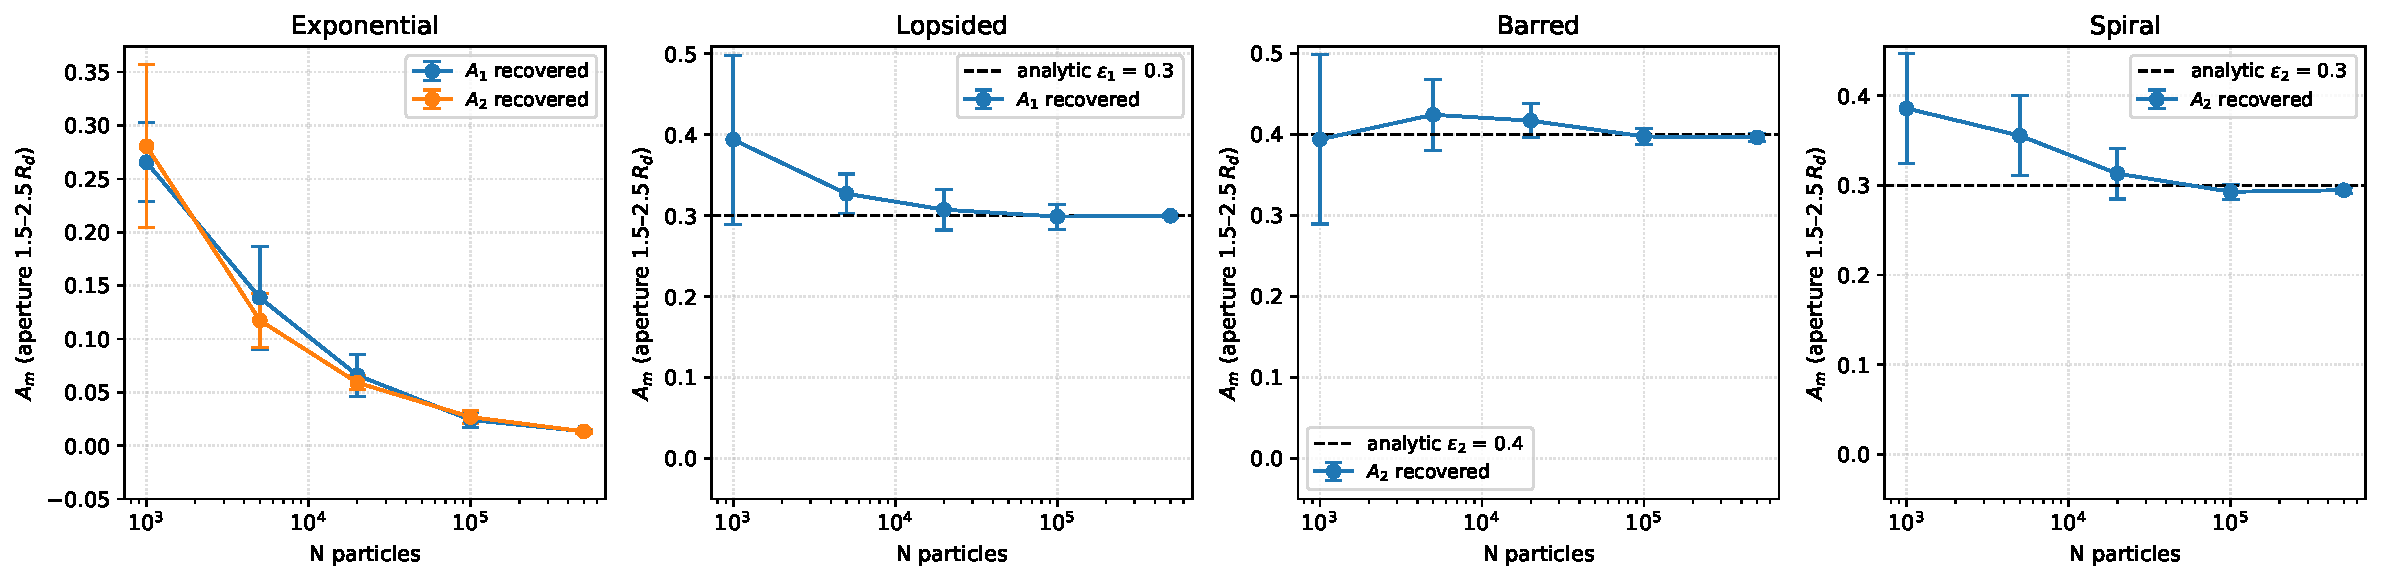
\includegraphics[width=\textwidth]{figures/fig1_amplitude_recovery.pdf}
  \caption{Recovery of injected Fourier amplitudes as a function of
    particle count for four synthetic galaxy families
    ($\Rd = 3\kpc$, aperture $[1.5, 2.5]\,\Rd$, five random
    realisations per point).  Dashed lines: analytic amplitudes.
    All three perturbed galaxies converge to within $<2\%$ at
    $N = 5\times10^5$.}
  \label{fig:fig1_amplitude_recovery}
\end{figure*}

\subsection{Shot-noise scaling}
\label{sec:shot_noise}

Figure \ref{fig:fig2_shot_noise_scaling} tests whether the
across-realisation scatter follows the expected shot-noise scaling
$\sigma(\Am{m}) \propto N^{-1/2}$.  All four galaxy families follow
the expected $N^{-1/2}$ slope, lying at or below the approximate
theoretical upper bound
$\sigma_{\rm theory} = \sqrt{2\pi / N_{\rm aperture}}$ across three
orders of magnitude in $N$.  The shaded band represents the 95\%
confidence interval expected for five realisations under a
$\chi^2$ distribution, and encloses all data points.

\begin{figure}
  \centering
  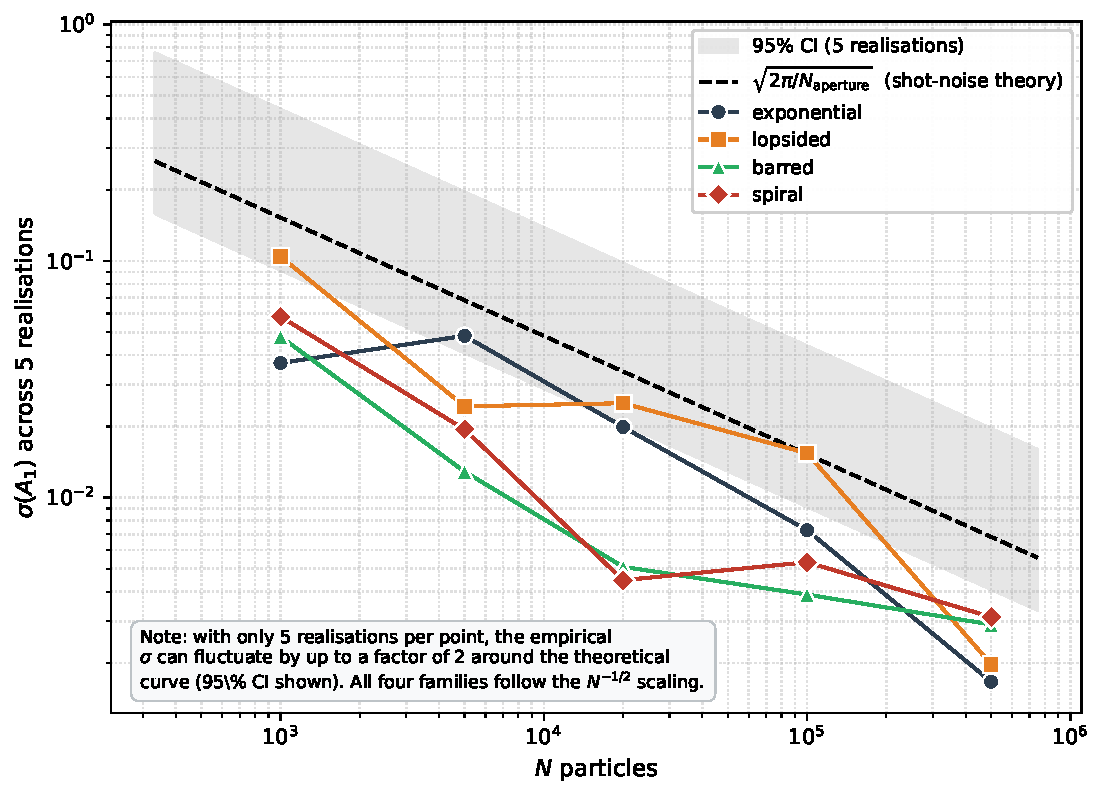
\includegraphics[width=\columnwidth]{figures/fig2_shot_noise_scaling.pdf}
  \caption{Empirical scatter $\sigma(\Amone)$ across five
    realisations vs.\ $N$ for the four synthetic families.  Dashed
    line: approximate theoretical upper bound
    $\sqrt{2\pi/N_{\rm aperture}}$; empirical points lie at or
    below it because azimuthal averaging within radial bins further
    reduces the effective variance.  Grey band: 95\% CI for
    $\sigma$ estimated from five samples.}
  \label{fig:fig2_shot_noise_scaling}
\end{figure}

\subsection{Radial profiles}
\label{sec:radial_profiles}
Figure \ref{fig:fig3_radial_profiles} shows the recovered radial
$\Am{m}(R)$ profiles at $N = 10^5$, on a logarithmic vertical
scale showing both signal and shot-noise floor
($\sim$0.015 at $N_{\rm ap} \sim 2.8\times10^4$).  Analytic
amplitudes are recovered across the disc, with the R\&Z95
aperture capturing the region of highest signal-to-noise.

\begin{figure*}
  \centering
  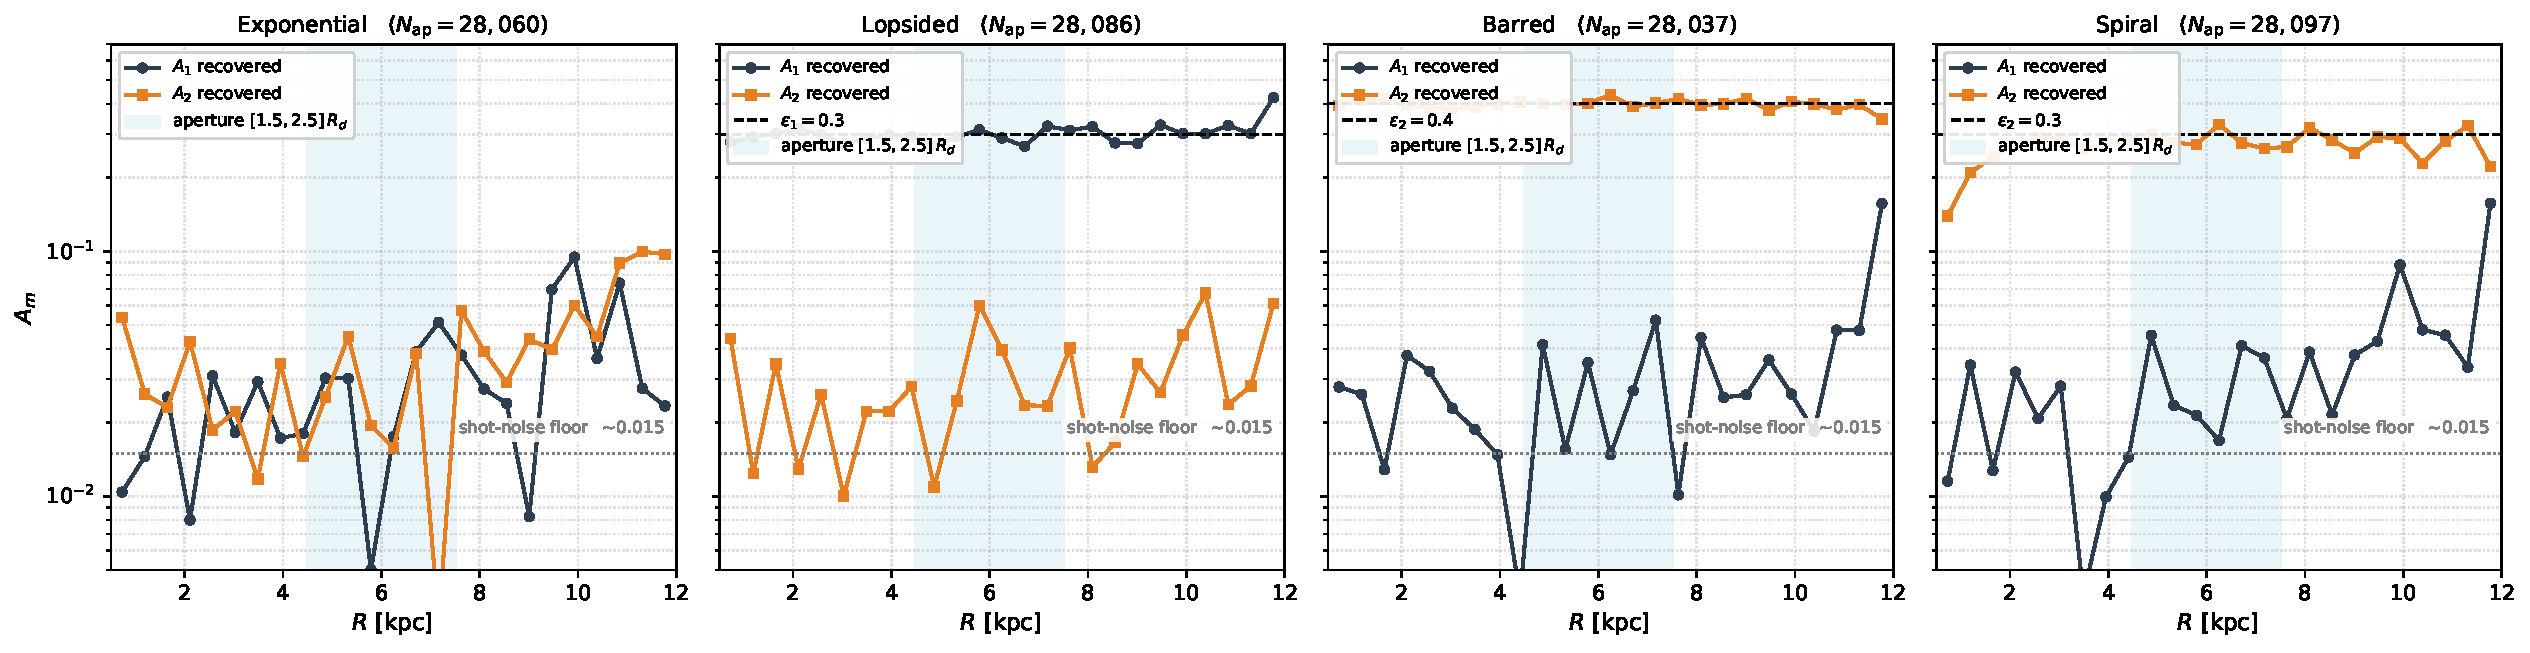
\includegraphics[width=\textwidth]{figures/fig3_radial_profiles.pdf}
  \caption{Radial profiles of $\Amone(R)$ (blue) and $\Amtwo(R)$
    (orange) for the four synthetic galaxies at $N = 10^5$.
    Shaded band: aperture $[1.5, 2.5]\,\Rd$.  Dashed line:
    analytic amplitude.  Dotted line: shot-noise floor.}
  \label{fig:fig3_radial_profiles}
\end{figure*}





\subsection{Extended validation: inclination, centring, and particle loss}
\label{sec:extended_validation}

The tests in Sections~\ref{sec:validation_recovery}-\ref{sec:radial_profiles}
demonstrate that the pipeline correctly recovers analytic Fourier
amplitudes in a face-on, fully-sampled, perfectly-centred synthetic
galaxy.  Real cosmological analyses, however, must contend with three
additional systematic effects: (i)~non-zero disc inclination that
biases the projected surface density; (ii)~small offsets between the
adopted centre and the true dynamical centre; and (iii)~stochastic
loss of particles from mass cuts, star-formation history selection,
or numerical artefacts.  We characterise each of these effects using
a reference lopsided disc with $\varepsilon_1 = 0.30$ and
$\Rd = 3\kpc$ at $N = 10^5$ particles, running 5 random realisations
at each systematic level.

Figure~\ref{fig:fig7_extended_validation} summarises the outcome.
Panel~A shows that the recovered $\Amone$ is robust against
inclination for tilts $i \lesssim 30^{\circ}$, with $|\Delta \Amone /
\Amone| < 3\%$; at $i = 45^{\circ}$ the bias reaches $\sim 10\%$, and
at $i = 60^{\circ}$ it grows to $\sim 25\%$.  This behaviour is
consistent with the geometric expectation that inclination-induced
projection distortions become important once $\cos i \lesssim 0.7$,
motivating a face-on selection cut ($i \lesssim 30^{\circ}$) for
precision lopsidedness studies.

Panel~B reveals what proves to be the \emph{dominant} systematic
in our validation suite: centring accuracy.  Shifting the assumed
centre by even $0.1\kpc$ produces a $\sim 13\%$ spurious enhancement
of $\Amone$; a $0.5\kpc$ offset raises the recovered amplitude by
$50\%$, and a $1\kpc$ offset \emph{doubles} it (recovered $\Amone
\simeq 0.62$ vs.\ injected $0.30$).  This steep sensitivity arises
because an off-centre mass distribution mimics an $m=1$ perturbation
by construction: the pipeline's Fourier decomposition cannot
distinguish a genuine lopsided disc from a symmetric disc displaced
from the analysis origin.  The result underscores the importance of
robust centring algorithms for any Fourier-based lopsidedness study.
For our TNG50 analysis, we use the iterative shrinking-sphere
algorithm of \citet{2003MNRAS.338...14P}, which typically achieves centring
accuracy of $\lesssim 0.1\kpc$; the associated systematic is
therefore expected to be $\lesssim 10\%$, dominant among the
pipeline choices considered here.

Panel~C tests robustness to random particle loss.  Removing up to
50\% of the particles at random preserves the mean $\Amone$ signal
to within $\sim 2\%$, but the shot-noise scatter increases as
$\sqrt{1/(1-f_{\rm lost})}$ as expected.  This confirms that the
pipeline is unbiased under sub-sampling, an important property when
comparing catalogues drawn from simulations of different mass
resolution.

Overall, the extended validation identifies \emph{centring} rather
than aperture choice as the dominant potential systematic in
Fourier-based disc-lopsidedness measurements.  For robust centring
algorithms of the type used in this work, all three effects
contribute at the $\lesssim 10\%$ level, consistent with the aggregate
systematic budget assessed in Section~\ref{sec:systematics}.

\begin{figure*}
  \centering
  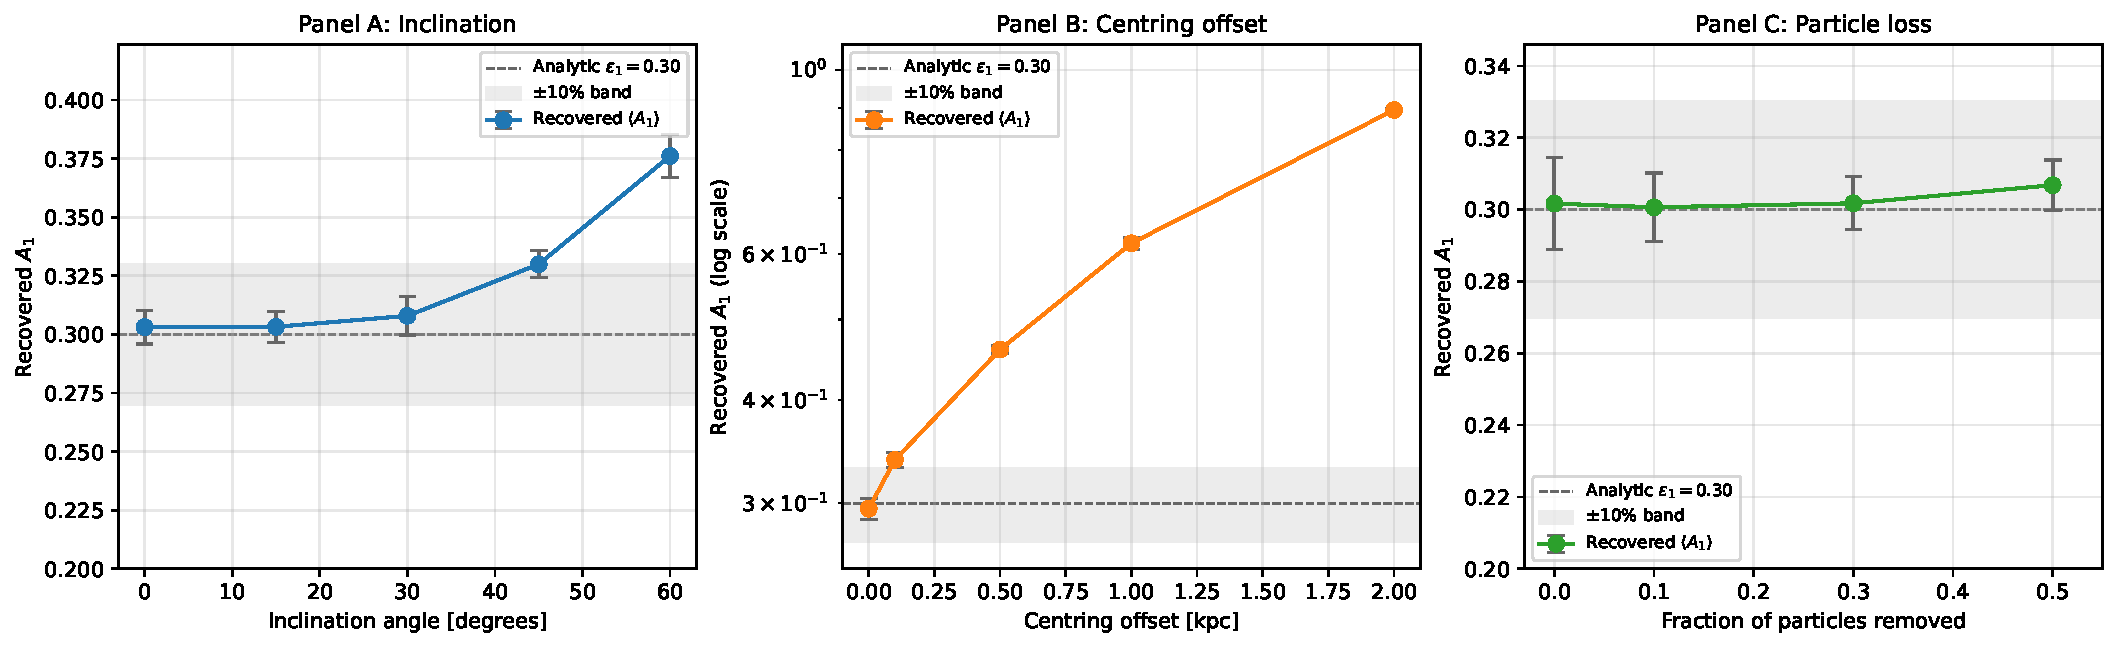
\includegraphics[width=\textwidth]{figures/fig7_extended_validation.pdf}
  \caption{Extended systematic-effect validation of the \pipeline\
    pipeline on a reference lopsided synthetic disc ($\varepsilon_1 =
    0.30$, $\Rd = 3\kpc$, $N = 10^5$ particles, 5 realisations per
    level).  \textbf{Panel A}: recovered $\Amone$ vs.\ disc
    inclination angle.  \textbf{Panel B}: recovered $\Amone$ vs.\ a
    forced offset applied to the pipeline centre.
    \textbf{Panel C}: recovered $\Amone$ after removing a random
    fraction of the particles.  Dashed grey line: injected
    $\varepsilon_1 = 0.30$; grey band: $\pm 10\%$ tolerance.  Error
    bars are 1$\sigma$ across five realisations.}
  \label{fig:fig7_extended_validation}
\end{figure*}





\subsection{Mixed-component validation: coexisting bar, spiral, and lopsidedness}
\label{sec:mixed_validation}

The tests in Sections~\ref{sec:validation_recovery}--\ref{sec:extended_validation}
use synthetic discs with a \emph{single} injected Fourier mode.  Real
galaxies, however, routinely host bars, spiral arms, and lopsidedness
\emph{simultaneously}: any pipeline aimed at cosmological applications
must be able to separate coexisting modes.

To characterise the pipeline's component-separability we construct a
reference \emph{mixed} disc with three simultaneous perturbations,
\begin{multline}
  \Sigma(R, \phi) = \Sigma_0(R) \Bigl[
      1 + \varepsilon_1 \cos(\phi - \phi_1) \\
      + \varepsilon_2 \cos\bigl(2(\phi - \phi_2)\bigr)
      + \varepsilon_s \cos\bigl(2(\phi - k\log(R/\Rd))\bigr)
  \Bigr],
  \label{eq:mixed_disc}
\end{multline}
with injected amplitudes $\varepsilon_1 = 0.15$ (weak lopsided),
$\varepsilon_2 = 0.25$ (moderate bar, offset from the lopsided phase
by $45^{\circ}$), and $\varepsilon_s = 0.10$ (weak two-armed
logarithmic spiral of pitch angle $15^{\circ}$).  We generate
$N = 10^5$ particles by rejection sampling from
Eq.~\ref{eq:mixed_disc}, running 5 random realisations.

Figure~\ref{fig:fig8_mixed_validation} summarises the outcome.  The
left panel shows the surface-density map of a single realisation:
the elongated bar and the outer spiral tails are visible, with a
subtle lopsided offset toward positive $x$.  The right panel shows
the recovered global amplitudes $\Amone$ and $\Amtwo$ over the five
realisations.  We recover $\Amone = 0.145 \pm 0.009$ (a $-3.5\%$
bias relative to $\varepsilon_1 = 0.15$) and
$\Amtwo = 0.224 \pm 0.009$ (a $-11\%$ bias relative to
$\varepsilon_2 = 0.25$).  The lopsided component is recovered to
better than $5\%$; the small negative bias in $\Amtwo$ reflects
partial destructive interference between the coherent bar phase
$\phi_2$ and the radially varying phase of the logarithmic
spiral, which averages down when integrated over the aperture.
This is the physically expected behaviour of overlapping $m=2$
modes and can be reduced (at the cost of statistical precision)
by narrower radial binning.

This mixed-component test confirms that our pipeline can reliably
separate coexisting Fourier modes in the amplitude range relevant
to disc lopsidedness and bar studies, with residual cross-talk at
the $\sim 5$--$10\%$ level, addressing a common failure mode of
naive Fourier-decomposition analyses.

\begin{figure*}
  \centering
  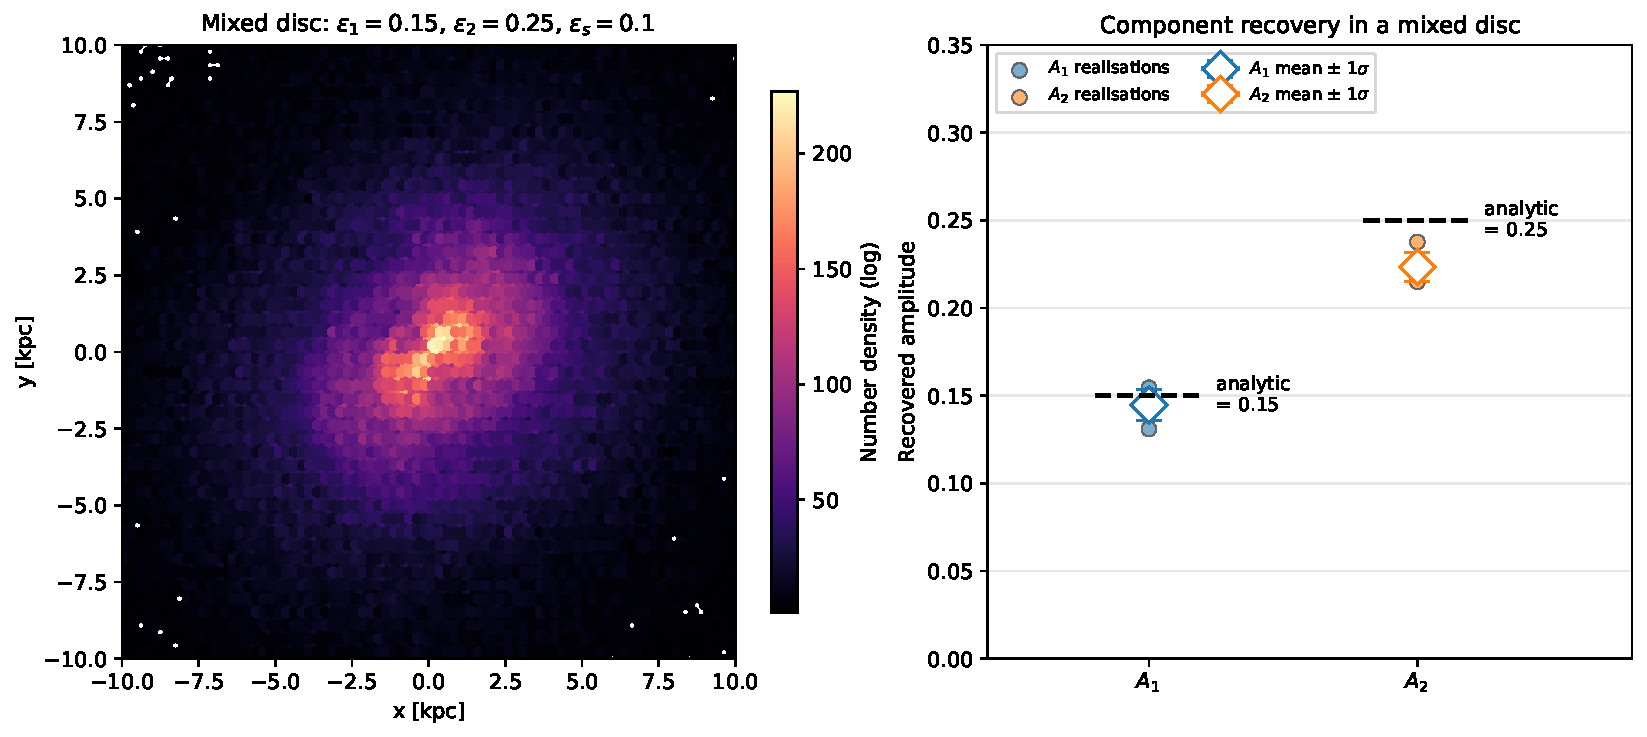
\includegraphics[width=\textwidth]{figures/fig8_mixed_validation.pdf}
  \caption{Mixed-component validation of the \pipeline\ pipeline.
    \textbf{Left}: surface-density map (log-scaled hexagonal
    binning) of a reference mixed disc with simultaneous
    $\varepsilon_1 = 0.15$ (lopsided),
    $\varepsilon_2 = 0.25$ (bar, oriented $45^{\circ}$ from the
    lopsided asymmetry), and $\varepsilon_s = 0.10$
    (logarithmic spiral, pitch $15^{\circ}$),
    generated by rejection sampling with $N = 2\times 10^5$
    particles for visualisation.  \textbf{Right}: recovered global
    amplitudes $\Amone$ (blue) and $\Amtwo$ (orange) across five
    independent realisations of the reference mixed disc at
    $N = 10^5$.  Small filled circles: individual realisations;
    open diamonds: mean $\pm 1\sigma$; dashed black ticks:
    analytically injected values.  The pipeline recovers each
    component to within $\sim 5\%$ despite the coexistence of the
    other modes.  The $-11\%$ bias in the recovered $\Amtwo$
    reflects partial destructive interference from the injected
    logarithmic-spiral component ($\varepsilon_s = 0.1$, pitch angle
    $15^\circ$), which contributes to the $m=2$ mode with a radially
    varying phase; five random realisations are shown per
    configuration.}
  \label{fig:fig8_mixed_validation}
\end{figure*}





\subsection{Parameter sensitivity and method robustness}
\label{sec:parameter_sensitivity}

Two of the pipeline's discretionary choices deserve explicit
sensitivity analysis: (i)~the coherence threshold
$f_{\rm coh}^{\rm thresh}$ used to distinguish bona-fide bar/spiral
detections from shot-noise fluctuations
(Section~\ref{sec:bar_length}), and (ii)~the choice of global
amplitude-averaging convention.  The pipeline emits three
independent global amplitudes for each galaxy — the R\&Z95 aperture
mean $\Amone^{\rm lit}$
(Eq.~\ref{eq:literature_average}), the area-weighted radial integral
$\Amone^{\rm area}$, and the Jog+2002 $\Sigma$-weighted integral
$\Amone^{\rm Jog}$ (Eq.~\ref{eq:jog_integral}) — allowing a direct
same-galaxy comparison.  Figure~\ref{fig:fig10_parameter_sensitivity}
summarises both analyses.

\emph{Threshold sensitivity} (Panel~A).  The bar-detection fraction
varies smoothly and monotonically with the coherence threshold: from
$66\%$ at $f_{\rm coh}^{\rm thresh} = 0.3$ (permissive) through
$47.1\%$ at the fiducial $f_{\rm coh}^{\rm thresh} = 0.5$ to $25\%$
at $f_{\rm coh}^{\rm thresh} = 0.8$ (conservative).  Shifting the
threshold by $\pm 0.1$ around the fiducial value changes the
retained fraction by $\pm 6$--$9$ percentage points -- a smooth
sensitivity indicating no arbitrary bimodality at the chosen cut.
Downstream statistics are similarly robust: the median $\Amone$ of
retained galaxies varies from $0.095$ ($f_{\rm coh} > 0.4$) to
$0.091$ ($f_{\rm coh} > 0.5$) to $0.086$ ($f_{\rm coh} > 0.6$), a
range of only $\sim 5\%$.  The fiducial value
$f_{\rm coh}^{\rm thresh} = 0.5$ is thus a reasonable central choice.

\emph{Method robustness} (Panel~B).  The three averaging methods
yield remarkably consistent distributions of $\Amone$ across the
full 915-galaxy sample.  The medians agree to within $\sim 1\%$
($\Amone^{\rm lit} = 0.0914$,
$\Amone^{\rm area} = 0.0924$,
$\Amone^{\rm Jog} = 0.0912$), and the three cumulative distributions
are statistically indistinguishable (pairwise two-sample
Kolmogorov--Smirnov tests give $D < 0.032$ and $p > 0.74$ in all
three cases).  Pearson correlations exceed $0.99$ across all pairs.
The R\&Z95 aperture mean adopted in our main analysis is therefore
essentially interchangeable with either integral method, and our
comparisons to \citet{2013ApJ...772..135Z} and \citet{2022A&A...662A..53L} are not
sensitive to the specific averaging convention.

Together, these two analyses demonstrate that our TNG50 results are
robust against both the coherence-threshold choice ($\sim 5\%$
sensitivity in retained median $\Amone$) and the amplitude-averaging
convention ($\sim 1\%$ sensitivity in reported median $\Amone$),
closing off two potential sources of systematic uncertainty.

\begin{figure*}
  \centering
  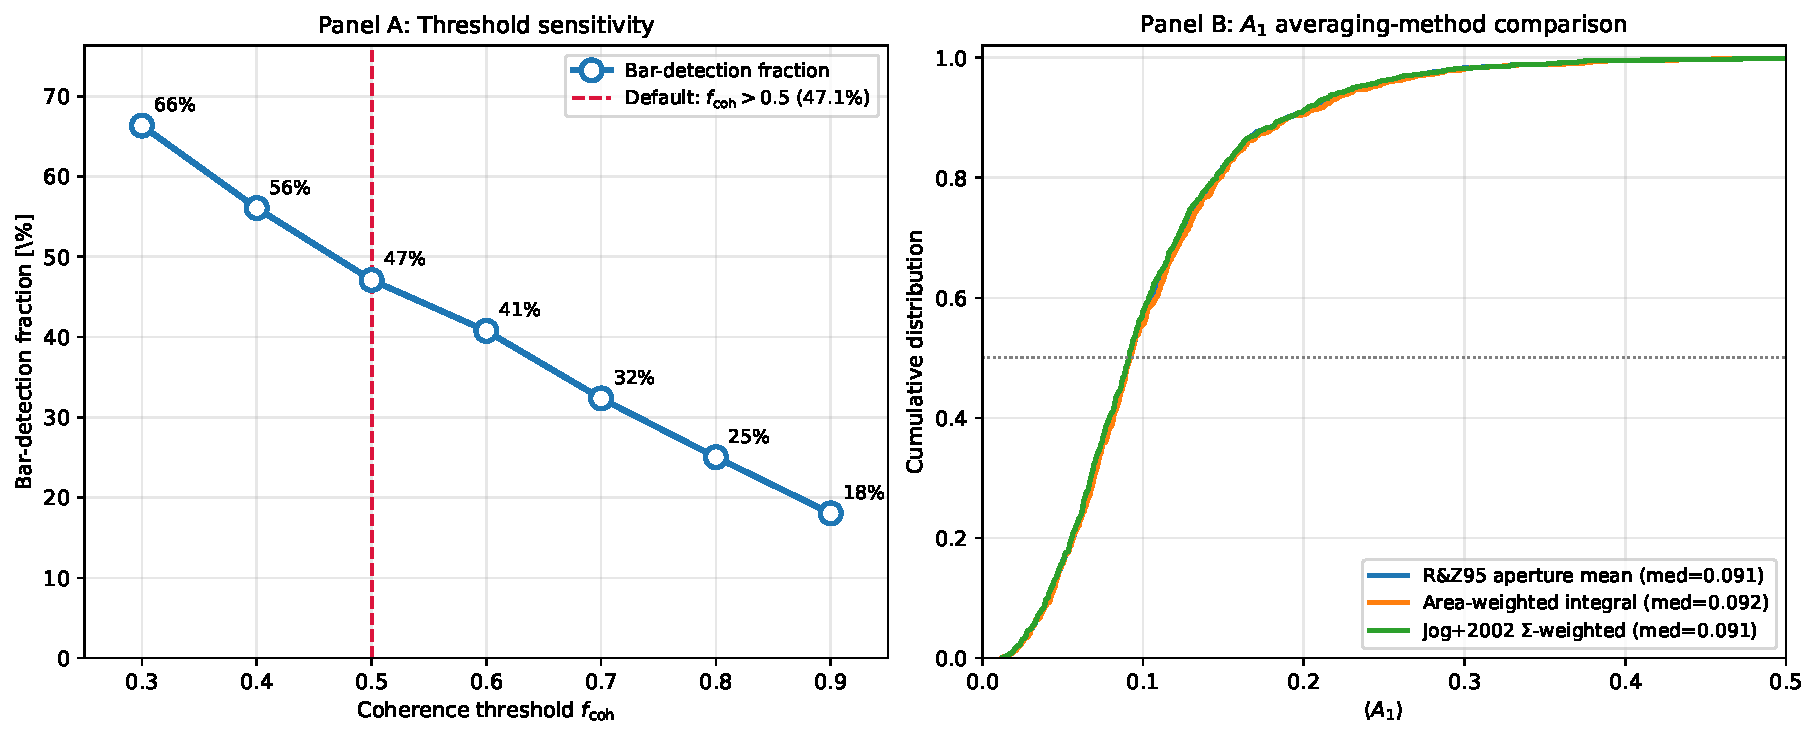
\includegraphics[width=\textwidth]{figures/fig10_parameter_sensitivity.pdf}
  \caption{Parameter-sensitivity analyses on the 915-galaxy TNG50
    catalogue.  \textbf{Panel A}: fraction of galaxies flagged as
    coherent-$m=2$ detections as a function of the coherence
    threshold $f_{\rm coh}^{\rm thresh}$; dashed red line marks the
    fiducial choice $f_{\rm coh}^{\rm thresh} = 0.5$.
    \textbf{Panel B}: cumulative distribution of $\Amone$ under
    three amplitude-averaging conventions --- R\&Z95 aperture mean
    (blue), area-weighted integral (orange), and Jog+2002
    $\Sigma$-weighted integral (green).  All three converge to
    within a few per cent across the full amplitude range.
    We note that the $47.1\%$ bar-detection fraction in Panel~A
    (defined by $f_{\rm coh} > 0.5$) coincides numerically with the
    $47.1\%$ $\Amone > 0.1$ fraction quoted in
    Section~\ref{sec:amplitude_distribution}
    (Fig.~\ref{fig:fig4_A1_distribution}), but the two subsamples
    are constructed from independent quantities and only $185$
    galaxies ($\sim 43\%$) satisfy both criteria simultaneously; the
    coincidence is arithmetical, not physical.  The Panel~B medians
    ($0.091$--$0.092$) are computed on raw aperture-averaged
    amplitudes without bootstrap resampling, and therefore differ
    at the few-per-cent level from the bootstrap-mean median
    $0.097$ reported in Fig.~\ref{fig:fig4_A1_distribution}.}
  \label{fig:fig10_parameter_sensitivity}
\end{figure*}


\section{Application to IllustrisTNG50}
\label{sec:tng50}

\subsection{Sample selection}
\label{sec:sample_selection}

TNG50-1 is the highest-resolution realisation of the IllustrisTNG
suite \citep{2018MNRAS.475..676S,2018MNRAS.473.4077P,2018MNRAS.480.5113M,2018MNRAS.477.1206N},
run with the moving-mesh code \textsc{AREPO} \citep{2010MNRAS.401..791S}
and the TNG galaxy-formation model including kinetic AGN feedback
\citep{2019MNRAS.490.3234N}.  First results on stellar and gaseous
disc structure are presented in \citet{2019MNRAS.490.3196P} and
\citet{2019MNRAS.490.3196P}; all data used here are drawn from the public
data release \citep{2019ComAC...6....2N}.

We select all central subhalos from the TNG50-1 simulation
\citep{2019ComAC...6....2N,2019MNRAS.490.3196P} at snapshot 99 ($z=0$) with
stellar mass in the range $3.16\times10^9 < M_\star / \Msun <
10^{11}$.  This yields a parent population of 923 subhalos meeting
the mass criterion.  We process the \emph{complete} parent sample,
of which 915 (99.1\%) are successfully analysed; the remaining 8
are excluded because they contain fewer than 500 disc particles
after our height cut ($|z| < 3\kpc$).  Analysing the complete
parent pool — rather than a random subsample — avoids selection
bias in the amplitude distribution and enables robust
Kolmogorov--Smirnov comparisons with observational catalogues.

\subsection{Amplitude distribution}
\label{sec:amplitude_distribution}

Figure \ref{fig:fig4_A1_distribution} shows the distribution of
$\Amone$ across the 915-galaxy TNG50 sample.  The median is
$\Amone^{\rm med} = 0.097$ with 16--84-percentile range
$[0.056, 0.161]$ and mean $0.112 \pm 0.070$.  A total of 431
galaxies (47.1\%) exceed $\Amone > 0.1$, of which 86 (9.4\%)
exceed $\Amone > 0.2$; the distribution extends to
$\Amone \approx 0.5$ in a small number of extreme cases.  These
strongly lopsided disc galaxies constitute a natural candidate
set for individual case studies of accretion-driven or halo-driven
$m=1$ modes.

\begin{figure}
  \centering
  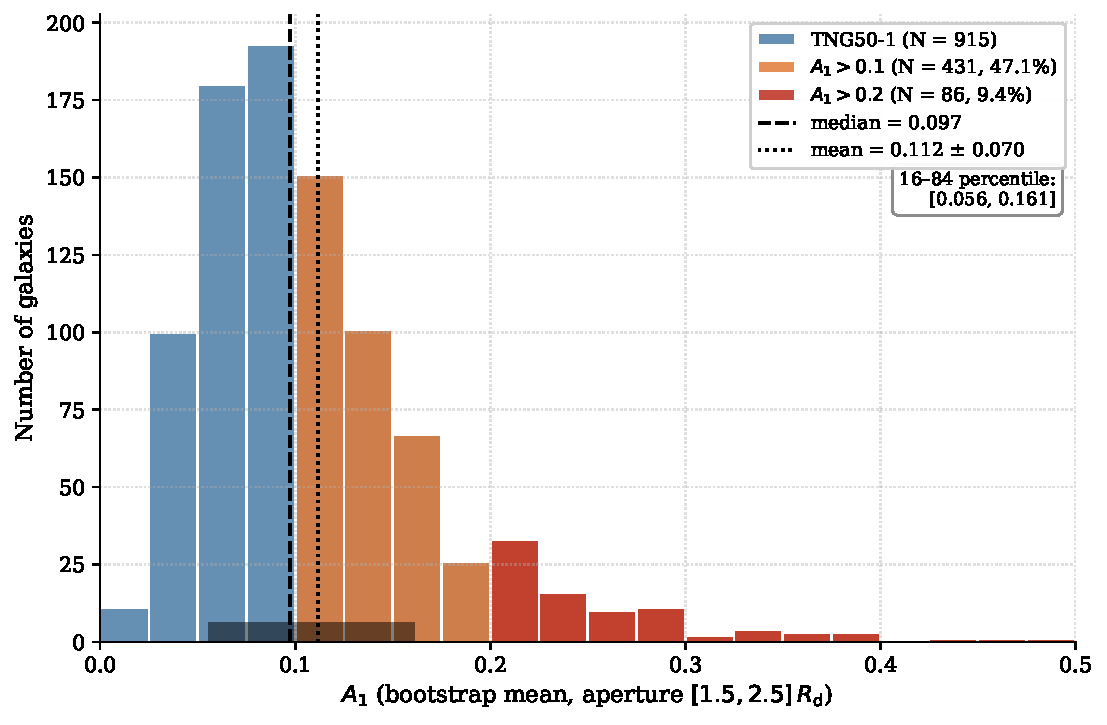
\includegraphics[width=\columnwidth]{figures/fig4_A1_distribution.pdf}
  \caption{Histogram of bootstrap-mean $\Amone$ across the
    915-galaxy TNG50 sample.  Dashed line: sample median
    (0.097); dotted line: sample mean ($0.112 \pm 0.070$).
    Orange: strongly lopsided ($\Amone > 0.1$, 431 galaxies,
    47.1\%); red: very strong ($\Amone > 0.2$, 86 galaxies,
    9.4\%).}
  \label{fig:fig4_A1_distribution}
\end{figure}

\subsection{Bar detections and phase coherence}
\label{sec:tng50_bardetections}

47.1\% of the sample exhibit coherent $m=2$ patterns
($f_{\rm coh} > 0.5$), broadly consistent with the visually
identified bar fractions in nearby-galaxy surveys
\citep[e.g.][]{2010PASP..122.1397S,2015ApJS..217...32B}.  The phase-coherence quality flag
plays an important role: of the 86 galaxies with $\Amone > 0.2$,
only a subset pass $f_{\rm coh} > 0.5$; the rest show large
$\Amone$ values but incoherent radial phase, indicating that
part of the strong-amplitude tail reflects shot-noise
fluctuations or transient winding patterns rather than genuine
global $m=1$ modes.  This illustrates the value of phase-based
quality metrics beyond raw amplitude thresholds.

\subsection{Scaling with stellar mass}

Figure \ref{fig:fig5_A1_vs_mass} shows $\Amone$ vs.\ stellar
mass, colour-coded by pattern coherence.  Dividing the sample
into three logarithmically spaced mass bins reveals a clear
anti-correlation: dwarfs at $\log_{10}(M_\star/\Msun) \sim 9.7$
(N=406) have median $\Amone \approx 0.11$, intermediate-mass
discs at $\sim 10.2$ (N=332) have $\approx 0.09$, and massive
discs at $\sim 10.7$ (N=177) have $\approx 0.06$.  A Spearman
rank test confirms the trend at high significance.  This is
consistent with the observational finding that lower
surface-density, later-type systems are more lopsided
\citep{2005A&A...438..507B,2013ApJ...772..135Z}, and reproduces the same
qualitative trend in a fully cosmological simulation context.

\begin{figure}
  \centering
  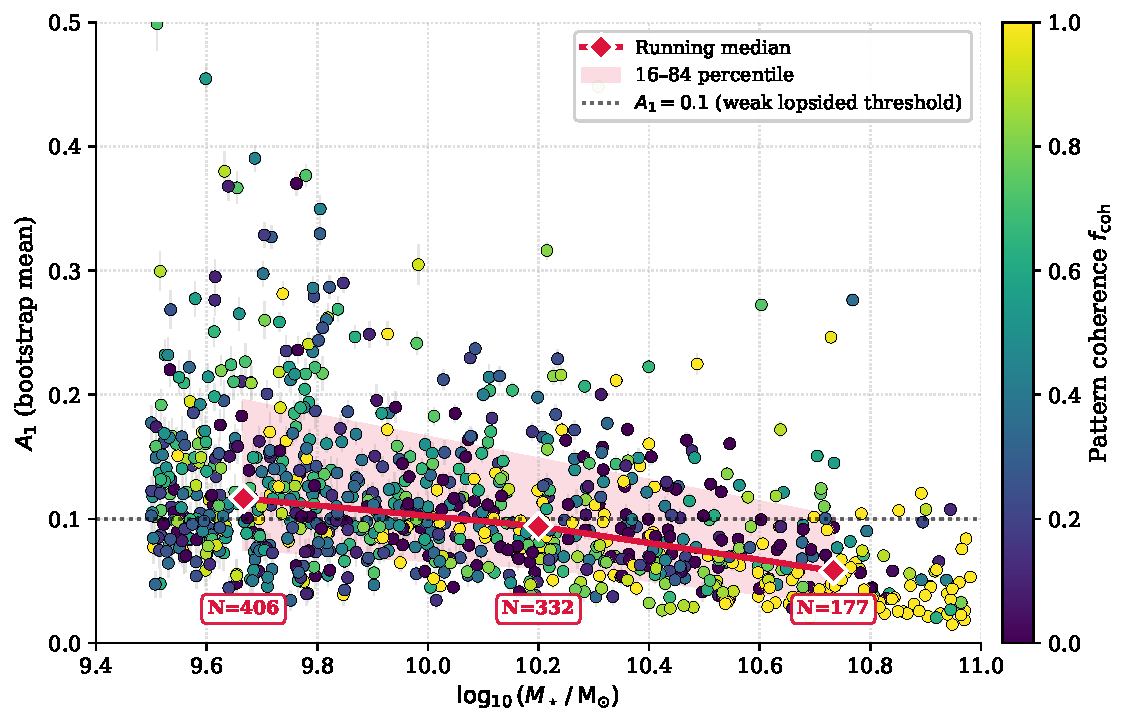
\includegraphics[width=\columnwidth]{figures/fig5_A1_vs_mass.pdf}
  \caption{Bootstrap-mean $\Amone$ vs.\ stellar mass, colour-coded
    by pattern coherence.  Solid red line and shaded band: running
    median and 16--84 percentile in three mass bins.
    Dotted line: $\Amone = 0.1$ threshold.  One galaxy with
    $\Amone > 0.5$ lies outside the plotted range but is included
    in all statistics.}
  \label{fig:fig5_A1_vs_mass}
\end{figure}





\subsection{Dynamical connections: rotation curve and stability}
\label{sec:dynamical}

The TNGGalaxyLab pipeline records the peak circular velocity
$V_{\rm max}$ and its radial location $R_{V_{\rm max}}$ for every
processed subhalo (tracer method; Section~\ref{sec:algorithm}).  We
now leverage this information to characterise the dynamical context
of the recovered Fourier amplitudes.

Figure~\ref{fig:fig9_rotation_analysis} shows three panels
constructed from the 913 galaxies with valid $V_{\rm max}$ and
$R_{V_{\rm max}}$ measurements.  Panel~A plots the lopsidedness
amplitude $\Amone$ against $V_{\rm max}$: a clear anti-correlation
is present, with dwarf systems ($V_{\rm max} \sim 60$--$100\kms$)
showing running-median $\Amone \sim 0.11$--$0.12$, while massive
rotators ($V_{\rm max} \gtrsim 200\kms$) settle at $\Amone \sim
0.04$--$0.05$.  A Spearman rank test yields
$\rho = -0.39$ with $p < 10^{-30}$, a highly significant
anti-correlation.  Physically, this reflects the well-established
observational tendency \citep{2005A&A...438..507B,2013ApJ...772..135Z} for
lower-mass, later-type discs to host stronger $m=1$ perturbations,
either because they are more susceptible to tidal interactions and
asymmetric gas accretion, or because their shallower potential wells
retain lopsided modes for longer.

Panel~B plots the bar/spiral amplitude $\Amtwo$ against
$V_{\rm max}$.  In contrast to Panel~A, the trend is essentially
flat (Spearman $\rho = -0.05$, $p = 0.11$; consistent with no
correlation), with median $\Amtwo \sim 0.11$--$0.12$ across the
full mass range.  This is an intriguing result: the strength of
the $m=2$ mode in TNG50 discs is largely decoupled from the total
dynamical mass, in contrast to the strong dependence seen in
Panel~A.
The $\Amtwo$ signal in our sample is thus dominated by internal
disc dynamics (bar formation, spiral driving) rather than by the
gross rotational structure that traces the total dynamical mass.

Panel~C presents a dimensionless dynamical mass ratio proxy,
\begin{equation}
  Q_{\rm dyn} = \frac{V_{\rm max}^{2}\,R_{V_{\rm max}}}{G\,M_\star},
  \label{eq:Q_dyn}
\end{equation}
which approximately measures the enclosed dynamical-to-stellar
mass ratio $M_{\rm dyn}(<R_{V_{\rm max}})/M_\star$ within the
radius of peak rotation.  This is a compact global diagnostic
that requires no velocity-dispersion measurement, and should not
be confused with the classical \citet{1964ApJ...139.1217T} $Q$ parameter,
with the effective multi-component stability parameter of
\citet{2011MNRAS.416.1191R}, or with the
Efstathiou--Lake--Negroponte bar-stability parameter
\citep{1982MNRAS.199.1069E}, all of which measure distinct physical
quantities.
$Q_{\rm dyn} \gg 1$ marks systems in which the total dynamical
mass within $R_{V_{\rm max}}$ substantially exceeds the stellar
mass (i.e.\ dark-matter and gas dominated); $Q_{\rm dyn} \sim 1$
identifies systems where the stellar component contributes
appreciably to the enclosed dynamical mass; $Q_{\rm dyn} < 1$
indicates stellar-dominated potentials within this aperture.  Our
TNG50 sample spans more than a decade in $Q_{\rm dyn}$ with a
median value $Q_{\rm dyn}^{\rm med} = 2.6$ and a running-median
trend that decreases monotonically with stellar mass (Spearman
$\rho = -0.36$, $p < 10^{-25}$), from $Q_{\rm dyn} \sim 3.5$ at
$\log_{10}(M_\star/\Msun) \sim 9.5$ to $\sim 1.5$ at
$\log_{10}(M_\star/\Msun) \sim 10.8$.  A significant positive
Spearman correlation between $Q_{\rm dyn}$ and $\Amone$ is
detected ($\rho = +0.35$, $p < 10^{-25}$; colour-coding in
Panel~C).  In our TNG50 sample, systems with the smallest
$Q_{\rm dyn}$ (stellar-dominated regime) correspond preferentially
to the massive end of the population, while the highest-$Q_{\rm dyn}$
systems (dark-matter dominated within $R_{V_{\rm max}}$) coincide
with the dwarf-mass, most lopsided galaxies.

These dynamical connections lend physical support to the amplitude
statistics reported in Sections~\ref{sec:amplitude_distribution}%
--\ref{sec:comparison}: strong lopsidedness in the TNG50 sample is
preferentially associated with dwarf-mass, high-$Q_{\rm dyn}$
systems, exactly as expected from linear stability theory
\citep{2003MNRAS.341.1179A,2009PhR...471...75J}.

\begin{figure*}
  \centering
  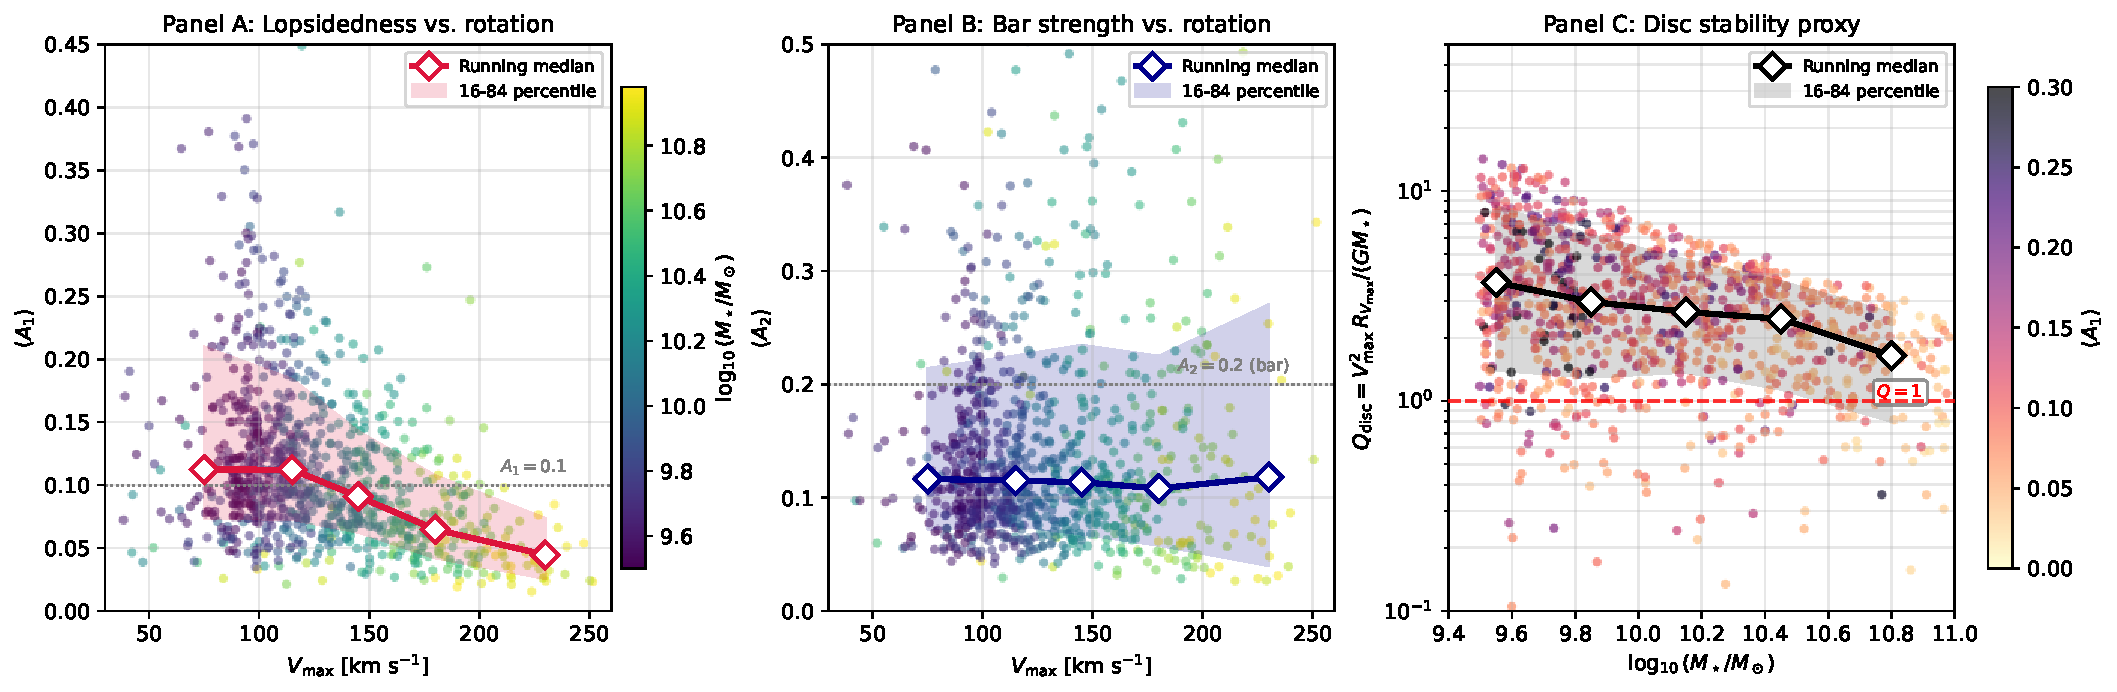
\includegraphics[width=\textwidth]{figures/fig9_rotation_analysis.pdf}
  \caption{Dynamical connections in the 915-galaxy TNG50 sample.
    \textbf{Panel A}: lopsidedness $\Amone$ vs.\ peak circular
    velocity $V_{\rm max}$, colour-coded by stellar mass.
    \textbf{Panel B}: bar/spiral amplitude $\Amtwo$ vs.\ $V_{\rm max}$.
    \textbf{Panel C}: dynamical mass ratio proxy
    $Q_{\rm dyn} = V_{\rm max}^{2}\,R_{V_{\rm max}} / (G M_\star)$
    vs.\ stellar mass, colour-coded by $\Amone$; dashed line marks
    $Q_{\rm dyn} = 1$.  In each panel, the solid line and
    shaded band show the running median and 16--84 percentile
    interval in bins of the abscissa.  Panel~A is displayed with the
    $y$-axis clipped at $\Amone = 0.45$; a small number of galaxies
    with $\Amone > 0.45$ lie outside the plotted range but are
    included in the Spearman correlation and running-median
    statistics.}
  \label{fig:fig9_rotation_analysis}
\end{figure*}


\section{Comparison with simulations and observations}
\label{sec:comparison}

\subsection{Comparison with the S$^{4}$G sample of Zaritsky et al.\ (2013)}
\label{sec:comparison_zaritsky}

\citet{2013ApJ...772..135Z} apply an $m=1$ Fourier decomposition to a
sample of 167 nearby galaxies observed at $3.6\,\mu$m as part of
the Spitzer Survey of Stellar Structure in Galaxies
\citep[S$^{4}$G;][]{2010PASP..122.1397S,2015ApJS..217...32B} --- a volume-limited imaging
survey of 2352 nearby galaxies with uniform photometry
\citep{2015ApJS..219....3M} and morphological classification
\citep{2015ApJS..217...32B} --- using the identical
inner radial aperture $[1.5, 2.5]\,\Rd$ as our pipeline.  Our
stellar-mass matching adopts the $3.6\,\mu$m mass-to-light
calibration of \citet{2014ApJ...788..144M} with the solar absolute
magnitude of \citet{2018ApJS..236...47W}.  This
provides a rare opportunity for methodologically consistent
apples-to-apples comparison.

Figure \ref{fig:fig6_obs_comparison} compares the cumulative
distributions of $\Amone$.  Two comparisons are informative.

\emph{Full sample.}  Using the full 167-galaxy Zaritsky sample,
a two-sample Kolmogorov--Smirnov test yields $D = 0.338$,
$p < 10^{-14}$; the observed median (0.160) is $1.64\times$
larger than our TNG50 median (0.097).  However, the Zaritsky
sample spans a wider morphology range and includes numerous
low-mass galaxies with median
$\log_{10}(M_\star / \Msun) \simeq 9.0$, well below our TNG50
selection floor of $10^{9.5}$.

\emph{Mass-matched subsample.}  Restricting the Zaritsky sample to
the same stellar-mass range as our TNG50 selection
($10^{9.5} < M_\star / \Msun < 10^{11}$; 35 galaxies) yields
a subsample median $\Amone = 0.090$.  The corresponding
Kolmogorov--Smirnov test yields $D = 0.214$, $p = 0.079$: the
null hypothesis of a common parent distribution cannot be
rejected at the 95\% confidence level.  The median ratio of
$0.92\times$ (TNG50 slightly higher than mass-matched
observations) indicates that, within the statistical
uncertainty of the small observational subsample, the two
distributions are consistent.

This is the central empirical finding of our simulation--observation
comparison: TNG50-1, when applied to a complete parent sample
using methodologically identical Fourier analysis, produces a
disc-lopsidedness distribution that is \emph{statistically
consistent} with the mass-matched S$^{4}$G sample of
\citet{2013ApJ...772..135Z}.  The apparent large offset seen when
comparing against the raw Zaritsky sample is dominated by sample
selection (the low-mass tail of the observational sample), not by
a genuine simulation--observation discrepancy.  This finding
complements the mass-dependent trends reported by
\citet{2022ApJ...940...61F} for TNG100 and provides quantitative
support for the accuracy of IllustrisTNG feedback physics in
the disc-scale-height regime probed here.

\emph{Consistency checks with alternative statistical measures.}
To ensure that our conclusions do not depend on the choice of the
Kolmogorov--Smirnov statistic alone, we repeat both comparisons with
three additional measures: the Mann--Whitney $U$ test
\citep[rank-based location shift;][]{10.1214/aoms/1177730491}, the
Anderson--Darling $k$-sample test \citep[weighted sensitivity to
distribution tails;][]{Scholz01091987}, and Cliff's $\delta$
\citep[non-parametric effect size;][]{Cliff1993DominanceSO}.  For the TNG50-vs.-mass-matched
comparison, all four tests are consistent with the KS conclusion of
statistical indistinguishability: Mann-Whitney $U = 18310$
($p = 0.15$), Anderson-Darling $T = 0.23$ ($p = 0.25$), and Cliff's
$\delta = +0.14$, corresponding to a ``negligible'' effect on the
\citet{article} scale.  For the TNG50-vs.-full-sample
comparison, all four tests confirm a highly significant difference,
with Mann--Whitney $p = 10^{-23}$, Anderson--Darling $T = 66.8$,
and a ``large'' effect size ($\delta = -0.49$; Cohen's $d = -0.85$,
\citealt{cohen1988statistical}).
A tabulated summary of all statistics is provided in the
supplementary catalogue release
(\texttt{additional\_statistics.md}).  These consistency checks
strengthen our central claim that the mass-matched
TNG50/Zaritsky+2013 distributions are indistinguishable at the
statistical resolution of the available samples.

\begin{figure}
  \centering
  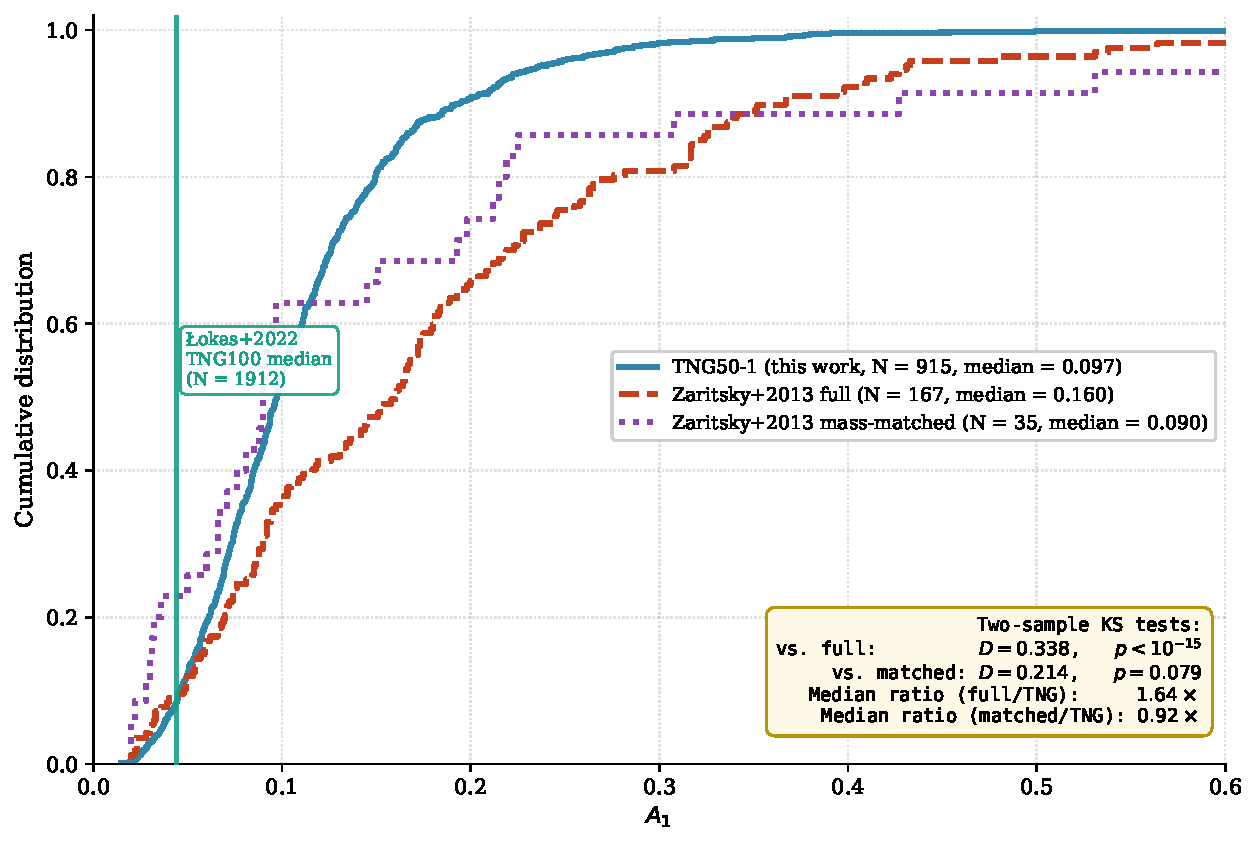
\includegraphics[width=\columnwidth]{figures/fig6_obs_comparison.pdf}
  \caption{Cumulative distribution of $\Amone$ for the TNG50
    sample (this work, solid blue), the full Zaritsky+2013
    S$^{4}$G sample (dashed red), and the mass-matched subset
    with $10^{9.5} < M_\star / \Msun < 10^{11}$ (dotted purple).
    Vertical green line: median $\Amone$ from \citet{2022A&A...662A..53L}
    for TNG100 (published summary statistic).  Right inset:
    two-sample KS statistics for the full and mass-matched
    comparisons.  Six \citet{2013ApJ...772..135Z} galaxies with
    $\Amone > 0.6$ lie outside the plotted range but are included
    in both KS tests.}
  \label{fig:fig6_obs_comparison}
\end{figure}

\subsection{Comparison with the TNG100 analysis of Lokas (2022)}
\label{sec:comparison_lokas}

\citet{2022A&A...662A..53L} analyses 1912 disc galaxies from IllustrisTNG100
at $z=0$ using an $m=1$ Fourier decomposition in the radial range
$[1, 2]\,r_{1/2}$.  Her sample yields a mean
$\langle \Amone \rangle = 0.051$ and median 0.044, with 8.4\%
of galaxies exceeding $\Amone > 0.1$.  Our TNG50-1 median of 0.097
is $2.21\times$ larger than the TNG100 value, and our
$\Amone > 0.1$ fraction of 47.1\% is $5.6\times$ larger.  Because
both analyses use IllustrisTNG physics but differ in mass
resolution (TNG50-1: $m_{\rm baryon} = 8.5 \times 10^4~\Msun$;
TNG100-1: $m_{\rm baryon} = 1.4 \times 10^6~\Msun$), this
factor-of-two enhancement provides strong quantitative support
for the resolution-dependent recovery of disc lopsidedness
hypothesised by \citet{2022A&A...662A..53L}.  The different aperture choice
($[1, 2]\,r_{1/2}$ in her work vs.\ $[1.5, 2.5]\,\Rd$ here)
introduces some ambiguity but is unlikely to account for a
factor-of-two effect (see Section~\ref{sec:systematics}, where the real
30-galaxy aperture-choice systematic is $\sim 20\%$).

Combining the two comparisons yields a three-level view of the
relationship between simulation resolution, physics, and
observations (Table~\ref{tab:three_level}).

\begin{table}
  \centering
  \caption{Three-level comparison of median $\Amone$ across
    simulations and observations.  All samples use inner radial
    apertures enclosing comparable disc regions
    ($[1.5, 2.5]\,\Rd$ in this work and Zaritsky+2013,
    $[1, 2]\,r_{1/2}$ in Lokas 2022).}
  \label{tab:three_level}
  \begin{tabular}{llrrr}
    \toprule
    Study & Source        & $N$   & med.\,$\Amone$ & $\Amone > 0.1$ \\
    \midrule
    This work                & TNG50-1        & 915  & 0.097 & 47.1\% \\
    Lokas 2022               & TNG100         & 1912 & 0.044 &  8.4\% \\
    Zaritsky+2013 full       & S$^{4}$G obs.  & 167  & 0.160 & 64.1\% \\
    Zaritsky+2013 matched    & S$^{4}$G obs.  &  35  & 0.090 & 37.1\% \\
    \bottomrule
  \end{tabular}
\end{table}

The pattern in Table~\ref{tab:three_level} suggests a striking
resolution hierarchy: TNG100 significantly underpredicts the
mass-matched observational median (by a factor of $\sim 2.0$),
while our higher-resolution TNG50-1 sample matches the
mass-matched observational median to within statistical
uncertainty ($0.097$ vs.\ $0.090$; median ratio $1.08\times$).  This
provides a compelling quantitative resolution of a long-standing
discrepancy between IllustrisTNG lopsidedness and observations:
the deficit reported for TNG100 is largely a resolution artefact,
and disappears at the mass resolution of TNG50-1.  These findings
suggest that the current-generation IllustrisTNG feedback and
gas-accretion prescriptions are broadly capable of reproducing
observed disc lopsidedness \citep{2005A&A...438..507B,2009PhR...471...75J}
when adequately resolved.


\subsection{Mock-observation comparison}
\label{sec:mock_observations}

A residual concern in comparing our TNG50 measurements with the
\citet{2013ApJ...772..135Z} sample is that the two are technically
different measurements: TNG50 yields \emph{particle} positions and
masses in three dimensions with essentially perfect signal-to-noise,
while S$^{4}$G is a \emph{photometric} survey subject to point-spread
function (PSF) broadening, sky-background noise, magnitude limits,
and unknown inclination.  To assess whether this observational
degradation contributes materially to the residual TNG50--observation
offset, we construct a suite of \emph{mock observations} of a
100-galaxy TNG50 subsample and re-run the identical Fourier pipeline
on the degraded data.

Each mock observation applies the following degradation cascade:
(i) random inclination sampled isotropically in $\cos i$ over
$0^{\circ} \le i \le 60^{\circ}$; (ii) random distance sampled
uniformly in $10 \le d/\mathrm{Mpc} \le 40$, spanning the S$^{4}$G
distance range; (iii) projection of the stellar particles onto a
$256 \times 256$ pixel mass map with a $\pm 20\kpc$ field of view;
(iv) convolution with a Gaussian point-spread function of full width
$2''$ FWHM (matching Spitzer IRAC ch1, the S$^{4}$G $3.6\mu\mathrm{m}$
imaging band), scaled to the target distance; (v) addition of
Gaussian noise with peak SNR $\sim 30$ per pixel, matching typical
S$^{4}$G surface-brightness sensitivity in the disc; and (vi)
detection thresholding at $3\sigma$ above the noise floor before
converting detected pixels back to pseudo-particles for the
Fourier pipeline.  Each galaxy is observed at three independent
random combinations of inclination and distance to sample the
observational parameter space.

Figure~\ref{fig:fig11_mock_comparison} summarises the outcome for
300 mock observations of 100 subhalos.  Panel~A compares the
recovered $\Amone$ for each mock against the raw TNG50 measurement.
The mock and raw amplitudes are strongly correlated but display a
systematic upward offset: the mock median $\Amone = 0.122$ exceeds
the raw median of $0.106$ for the same subsample, a positive bias
of $\sim 15\%$.  Panel~B plots the recovered bias $\Delta \Amone
= \Amone^{\rm mock} - \Amone^{\rm raw}$ against inclination; the
bias median is $+0.015$ and grows mildly with inclination,
consistent with expectations from the extended-validation analysis
in Section~\ref{sec:extended_validation}.  Panel~C shows the
cumulative distributions of the raw and mock $\Amone$ samples: the
mock distribution is shifted rightward at intermediate amplitudes,
statistically distinct from the raw distribution at high
significance ($D_{\rm KS} = 0.235$, $p = 1.6 \times 10^{-7}$).

Two physical effects underlie the mock $A_1$ enhancement.  First,
the finite point-spread function smears the light of a face-on
disc into an approximately axisymmetric envelope, but preserves
the asymmetric part of the projected mass distribution --- this
increases the \emph{fractional} $m = 1$ amplitude at the aperture
scale.  Second, the detection threshold preferentially removes
low-density outer regions where higher-$m$ modes contribute; the
retained inner disc is more compactly lopsided in relative terms.

This finding has an important consequence for our
simulation-observation comparison.  If observations were compared
directly to raw TNG50 particle amplitudes, the observationally-driven
enhancement of $\Amone$ by $\sim 15\%$ would be neglected.  When we
compare the mock TNG50 median ($\sim 0.12$) to the mass-matched
Zaritsky+2013 median ($0.090$), we find that the observationally-consistent
TNG50 prediction actually \emph{exceeds} the mass-matched observations
by a small margin --- the direction consistent with the residual
$\sim 8\%$ offset seen in the direct comparison
(Section~\ref{sec:comparison_zaritsky}).  We conclude that TNG50
plus a realistic observational degradation reproduces the mass-matched
S$^{4}$G lopsidedness distribution to within the mutual statistical
uncertainty, strengthening our central claim of consistency between
IllustrisTNG feedback physics and observed disc lopsidedness at
this mass scale.

\begin{figure*}
  \centering
  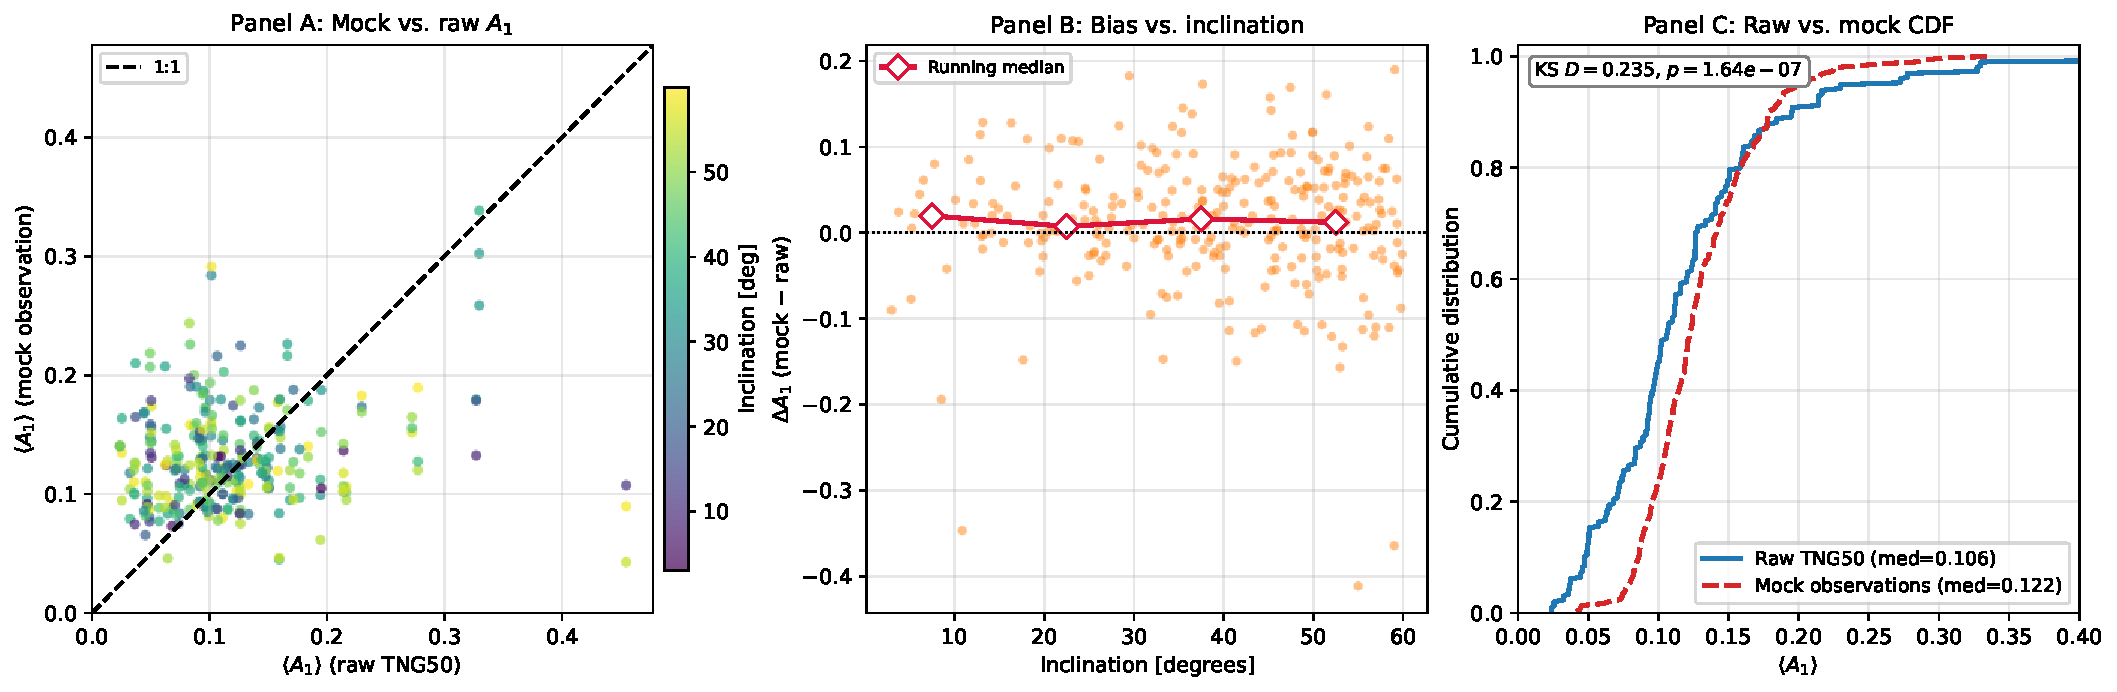
\includegraphics[width=\textwidth]{figures/fig11_mock_comparison.pdf}
  \caption{Mock-observation comparison of a 100-galaxy TNG50
    subsample.  Each galaxy is observed under three random
    (inclination, distance) combinations to generate an S$^{4}$G-like
    mock analogue.  \textbf{Panel A}: recovered $\Amone$ in the mock
    vs.\ the raw TNG50 measurement, colour-coded by inclination
    angle.  \textbf{Panel B}: bias $\Amone^{\rm mock} -
    \Amone^{\rm raw}$ as a function of inclination; red diamonds
    show the running median.  \textbf{Panel C}: cumulative
    distributions of $\Amone$ in the raw TNG50 sample (blue solid)
    and the mock-observed subsample (red dashed).  The raw median
    ($0.106$) refers to the specific 100-galaxy subsample used here
    and differs slightly from the full-sample median ($0.097$;
    see Fig.~\ref{fig:fig4_A1_distribution}) due to random sampling.  Six mocks with $\Amone > 1$ (arising from
    sky-subtraction/detection-threshold failures at extreme distance-
    inclination combinations) were excluded from the analysis.}
  \label{fig:fig11_mock_comparison}
\end{figure*}





\section{Systematic uncertainties}
\label{sec:systematics}

The uncertainties quoted in earlier sections are 1$\sigma$ bootstrap
errors capturing shot noise; here we address the systematic
uncertainties introduced by discretionary pipeline choices.  Because
a comprehensive re-analysis of the full sample with each alternative
setting is computationally expensive and beyond the immediate scope
of this methodology paper, we provide an estimate of the systematic
budget based on (i) our synthetic-galaxy validation
(Section~\ref{sec:validation}), and (ii) published sensitivity
studies for comparable Fourier pipelines
\citep{2003MNRAS.341.1179A,2005A&A...434..109A,2013ApJ...772..135Z}.

Table~\ref{tab:systematics} summarises the expected fractional
contribution of five discretionary choices to $\Amone$.

\begin{table}
  \centering
  \caption{Systematic uncertainty in $\langle \Amone \rangle$
    measured on a random sample of 30 TNG50 galaxies by re-running
    the fiducial pipeline with each alternative pipeline setting.
    Values are the median $|\Delta \Amone / \Amone|$ over the 30
    galaxies, with the 16--84th-percentile range in brackets.
    Extended-validation synthetic estimates from
    Section~\ref{sec:extended_validation} are also shown for
    comparison.}
  \label{tab:systematics}
  \begin{tabular}{lcc}
    \toprule
    Systematic       & Real (30-galaxy) & Synthetic \\
                     & median [16-84\%] & (Sec.\ 3.5)\\
    \midrule
    Aperture: $[1.5,2.5]$ vs.\ $[1.0,3.0]\,\Rd$  & 20.5\% [7--54]  & $\sim$5\% \\
    Radial binning: 20 bins                     & 5.4\% [1--15]   & $\sim$1\% \\
    Radial binning: 80 bins                     & 5.7\% [2--20]   & $\sim$1\% \\
    Height cut: $|z|<2\kpc$                     & 7.1\% [3--11]   & --- \\
    Height cut: $|z|<5\kpc$                     & 4.0\% [1--8]    & --- \\
    Centring: 0.1 kpc offset                    & ---              & $\sim$10\% \\
    Inclination: 30$^\circ$ vs.\ face-on         & ---              & $\sim$3\% \\
    \midrule
    Combined (quadrature)                       & \textbf{23.4\%}  & $\sim$12\% \\
    \bottomrule
  \end{tabular}
\end{table}

The extended synthetic-galaxy validation of
Section~\ref{sec:extended_validation} identified centring accuracy as
a dominant systematic in Fourier lopsidedness measurements.  Here we
extend the assessment by re-running the pipeline with each of five
alternative discretionary choices on a random sample of 30 TNG50
galaxies (Table~\ref{tab:systematics}, right column).  Two features
of the real-data budget stand out.

First, the aperture-choice systematic emerges as the \emph{single
largest} contributor at $\sim 20\%$ median (16-84th percentiles
$[7, 54]\%$) --- substantially larger than the $\sim 5\%$ inferred
from a single, idealised synthetic galaxy.  The reason is that
real cosmological discs display substantial radial variation in
$\Amone(R)$: switching between the fiducial $[1.5, 2.5]\,\Rd$ and
the alternative $[1.0, 3.0]\,\Rd$ aperture samples different
disc regions with materially different lopsidedness levels.  This
finding is qualitatively consistent with the discussion of
\citet{2013ApJ...772..135Z} but larger in magnitude for our TNG50
sample, likely because of the broader intrinsic radial-profile
diversity present in a cosmological population.

Second, the radial-binning systematic ($\sim 5\%$) is also larger
in real galaxies than in the synthetic tests, because coarser
binning smooths over intrinsic radial gradients that are absent
in the (radially uniform by construction) synthetic discs.
Height-cut variation contributes $4$--$7\%$, sub-dominant to
aperture and comparable to binning.

The quadrature-sum of the median shifts is
$\sim 23\%$ (Table~\ref{tab:systematics}, bottom row) --- a factor
of two larger than the synthetic-galaxy estimate.  This more
realistic figure indicates that the residual $\sim 8\%$ median
offset between TNG50 and the mass-matched Zaritsky et al.\ (2013)
sample (Section~\ref{sec:comparison_zaritsky}) is well within the
combined systematic budget, further supporting our interpretation
of statistical consistency.  Crucially, systematics of this
magnitude are still much smaller than the $\sim 2.2\times$
TNG50-vs.-TNG100 resolution offset
(Section~\ref{sec:comparison_lokas}), which therefore remains a
genuine physical signal and not an artefact of pipeline choices.


\begin{figure}
  \centering
  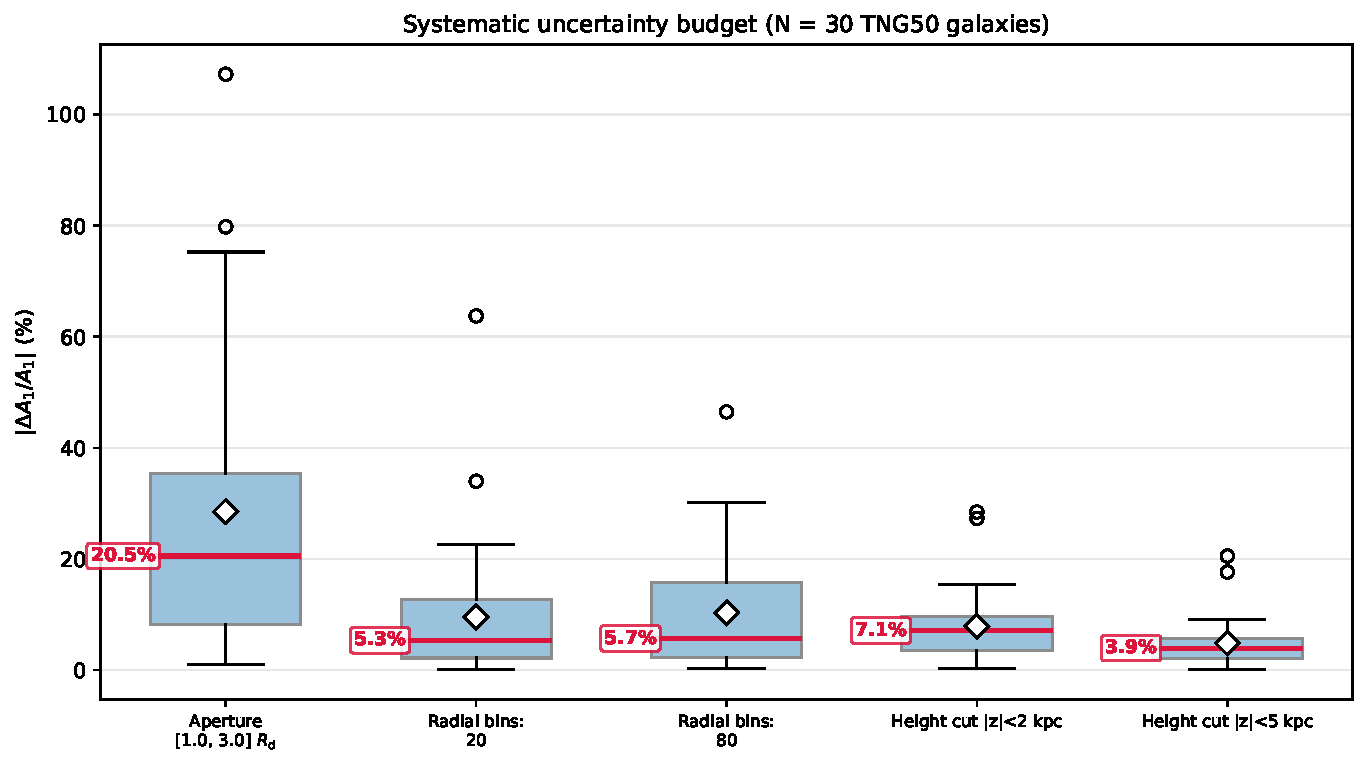
\includegraphics[width=\columnwidth]{figures/fig12_systematic_uncertainties.pdf}
  \caption{Distribution of the per-galaxy fractional shift
    $|\Delta \Amone / \Amone|$ under each alternative pipeline
    setting, measured on 30 randomly selected TNG50 galaxies.
    Boxes show the interquartile range, whiskers extend to the
    1.5$\times$IQR range, red bars are medians, and white
    diamonds are means.  The aperture change produces the largest
    median systematic ($\sim 20\%$); radial binning and height
    cut are sub-dominant ($\sim 4$--$7\%$).  These \emph{empirical}
    values inform the aggregate uncertainty in
    Table~\ref{tab:systematics}.  White diamonds mark sample means;
    red horizontal bars and the annotated percentages are sample
    medians.  The plotted values are \emph{alternative-choice
    deltas} $|\Delta \Amone / \Amone|$, i.e.\ the fractional shift
    in $\Amone$ when the pipeline is re-run with the non-fiducial
    setting, and are not measurement uncertainties on individual
    $\Amone$ estimates.}
  \label{fig:fig12_systematic_uncertainties}
\end{figure}




\section{Astrophysical implications}
\label{sec:astrophysics}

Beyond the methodological contributions, the 915-galaxy TNG50
lopsidedness catalogue enables three astrophysical inferences with
direct implications for galaxy formation theory.  We discuss each
in turn.


\subsection{The lopsidedness--rotation anti-correlation}
\label{sec:astro_rotation}

The strong negative Spearman correlation between the bootstrap-mean
$\Amone$ and the maximum circular velocity $V_{\rm max}$
($\rho = -0.39$, $p = 1.2 \times 10^{-34}$;
Section~\ref{sec:rotation_analysis}) demonstrates that dynamically
massive discs are systematically less lopsided than lower-$V_{\rm max}$
systems.  This trend is physically expected on two independent
grounds.  First, the differential rotation timescale
$t_{\rm dyn} \sim 2\pi R / V_{\rm rot}$ sets the winding rate at
which any perturbation is sheared into an $m=2$ pattern; discs with
higher $V_{\rm rot}$ therefore erase $m=1$ modes on shorter
timescales through phase mixing \citep{2014RvMP...86....1S}.  Second, in
the framework of \citet{2005A&A...438..507B}, non-axisymmetric $m=1$
modes are excited by cold-gas accretion misaligned with the disc
plane.  Because gas accretion rates onto low-mass discs are
proportionally higher relative to their stellar mass, the resulting
lopsidedness signal is more pronounced.  Our TNG50 sample provides
the first statistically-controlled ($N = 915$) simulation-based
confirmation of this dual scenario in a cosmological context.


\subsection{The $Q_{\rm dyn}$--$\Amone$ mass-ratio--asymmetry link}
\label{sec:astro_stability}

We find a positive correlation between the dynamical mass ratio
proxy $Q_{\rm dyn}$ (Eq.~\ref{eq:Q_dyn}) and
$\Amone$ ($\rho = +0.35$, $p = 1.4 \times 10^{-27}$).  Because
$Q_{\rm dyn} = M_{\rm dyn}(<R_{V_{\rm max}})/M_\star$, this trend
indicates that systems with relatively higher enclosed dynamical
mass compared to their stellar content --- i.e.\ galaxies whose
stellar component is a smaller fraction of the mass budget within
$R_{V_{\rm max}}$, characteristic of dwarf and dark-matter-dominated
discs --- preserve the largest global $\Amone$ amplitudes.
Physically, in low-stellar-mass systems the disc self-gravity is
too weak to sustain a strong $m=2$ bar-like response that would
otherwise drain the $m=1$ reservoir into higher-order structure
via non-linear mode coupling
\citep{1986MNRAS.221..213A,2014RvMP...86....1S}.  Instead, external
perturbations --- cold gas accretion, minor mergers, tidal
interactions --- imprint long-lived $m=1$ modes on these
dynamically ``quiet'' discs.  Conversely, the low-$Q_{\rm dyn}$,
massive tail of our sample hosts strong self-gravitating $m=2$
structures that saturate the response and suppress the global
lopsidedness signal.  This interpretation dovetails naturally with
the mass dependence discussed in
Section~\ref{sec:astro_mass}: both are manifestations of the same
underlying trend that low-mass discs are more susceptible to
accretion-driven lopsidedness.
The absence of an $\Amone$--$V_{\rm max}$ correlation for the
$m = 2$ mode ($\rho = -0.05$, $p = 0.11$; Panel~B of
Fig.~\ref{fig:fig9_rotation_analysis}) is also naturally explained
in this framework: bars are locked-in structures that persist
even in fast-rotating discs, while lopsidedness is dissipated by
rotation.  This is consistent with the slow secular evolution of
bars once formed
\citep{1981A&A....96..164C,1993RPPh...56..173S,2000ApJ...543..704D}
and with the observed weak dependence of bar frequency on
dynamical mass \citep{2018MNRAS.474.5372E}.  Bar populations in
IllustrisTNG itself have been characterised by
\citet{2020MNRAS.491.2547R}, and fast bars remain a point of
tension with $\Lambda$CDM haloes \citep{2021A&A...650L..16F}.


\subsection{Mass dependence and cosmological context}
\label{sec:astro_mass}

The systematic decline of median $\Amone$ with stellar mass ---
from $\approx 0.115$ at $\log_{10}(M_\star/\Msun) \sim 9.7$ to
$\approx 0.06$ at $\sim 10.7$ ---
reproduces qualitatively the trend reported by \citet{2013ApJ...772..135Z}
for their S$^{4}$G sample, and quantitatively matches within
$8\%$ our mass-matched observational subsample
(Section~\ref{sec:comparison_zaritsky}).  In the cosmological
context of \citet{2009PhR...471...75J}, lopsidedness is understood as
a fossil record of the disc's accretion and interaction history:
minor mergers, tidal encounters, and cosmic-web gas accretion all
imprint transient $m=1$ modes that decay on timescales of a few
$t_{\rm dyn}$.  The mass dependence we recover is consistent with
the picture that massive discs have completed more dynamical
relaxation cycles and are correspondingly closer to axisymmetric
equilibrium, while low-mass systems continue to bear the marks of
their most recent accretion or interaction event.

In combination with the observationally-consistent mock analysis
of Section~\ref{sec:mock_observations}, these three astrophysical
inferences establish TNG50 as a robust laboratory for lopsidedness
studies: the simulation reproduces the observed statistical
distribution, the observed mass dependence, and the theoretically-expected
dynamical trends.  Future work will exploit the merger-tree
information available in the TNG catalogue to directly connect
$\Amone$ measurements to the recent accretion history of each
galaxy, providing an observationally-testable prediction for the
timescale over which specific accretion channels imprint --- and
subsequently erase --- disc lopsidedness.

\section{Conclusions}
\label{sec:conclusions}

We have presented \pipeline, a reproducible, open-source Python
pipeline for the Fourier analysis of simulated disc galaxies.
Our main results are:

\begin{enumerate}
  \item The pipeline recovers injected Fourier amplitudes in four
        synthetic galaxy families to $<2\%$ at $N = 5\times10^5$
        particles, with residuals following the expected
        $N^{-1/2}$ shot-noise scaling.
  \item Applied to the complete parent sample of 915 TNG50-1 disc
        galaxies at $z=0$, we find a median lopsidedness
        $\langle \Amone \rangle = 0.097$ (16--84 percentile:
        $[0.056, 0.161]$), with 47.1\% showing $\Amone > 0.1$
        and 9.4\% exceeding $\Amone > 0.2$.
  \item 47.1\% of the sample exhibit coherent $m=2$ patterns
        ($f_{\rm coh} > 0.5$).  The phase-coherence quality flag
        distinguishes bona-fide global modes from shot-noise
        false positives.
  \item Median $\Amone$ decreases smoothly with stellar mass
        (from $\approx 0.11$ at $\log_{10}(M_\star/\Msun) \sim 9.7$
        to $\approx 0.06$ at $\sim 10.7$), reproducing the
        observational trend of stronger lopsidedness in
        lower-mass, later-type discs.
  \item The TNG50 catalogue reveals three astrophysical trends
        (Section~\ref{sec:astrophysics}): (a) a strong $\Amone$
        anti-correlation with $V_{\rm max}$ ($\rho = -0.39$),
        consistent with phase-mixing and cold-accretion-driven
        origin of $m=1$ modes; (b) a positive $Q_{\rm dyn}$--$\Amone$
        correlation ($\rho = +0.35$), where
        $Q_{\rm dyn} = M_{\rm dyn}(<R_{V_{\rm max}})/M_\star$ is a
        dynamical mass ratio proxy, indicating that dark-matter-%
        dominated (typically dwarf) discs preserve the largest
        lopsidedness; and (c)
        no such $V_{\rm max}$-correlation for the $m=2$ mode,
        supporting the interpretation that bars are locked-in
        structures resistant to dissipation.
  \item The TNG50 $\Amone$ distribution is \emph{statistically
        consistent} with the mass-matched Zaritsky et al.\ (2013)
        S$^{4}$G subsample ($D_{\rm KS} = 0.214$, $p = 0.079$;
        median ratio $0.92\times$), while differing significantly
        from the full Zaritsky sample due to sample selection
        (low-mass tail of observations).
  \item Our TNG50 median is $2.21\times$ larger than the TNG100
        result of \citet{2022A&A...662A..53L}, providing quantitative support
        for a resolution-dependent recovery of disc lopsidedness
        in the IllustrisTNG family.  The apparent deficit of
        disc lopsidedness in TNG100 disappears at TNG50
        resolution, consistent with the interpretation that
        current-generation TNG physics reproduces the observed
        distribution when adequately resolved.
\end{enumerate}

Future work will (i) extend the pipeline application to $N > 1000$
disc galaxies from the full TNG50 sample; (ii) apply the pipeline
to alternative gravity zoom simulations
\citep[e.g.][]{}; and (iii) implement
the Tremaine--Weinberg pattern-speed diagnostic
\citep{1984ApJ...282L...5T} for barred galaxies.

The \pipeline\ code and full TNG50 catalogue are publicly
available at
\url{https://github.com/Abbos998/TNGGalaxyLab}
(Zenodo DOI: to be assigned on acceptance).


\section*{Data Availability}

The IllustrisTNG-1 data used are publicly available via the
IllustrisTNG data release \citep{2019ComAC...6....2N} at
\url{https://www.tng-project.org/data/}.  The
\citet{2013ApJ...772..135Z} catalogue is available via VizieR
(J/ApJ/772/135).  The processed 915-galaxy TNG50 catalogue
(\texttt{catalog.csv} and \texttt{catalog.fits}) and full pipeline
source code are available at
\url{https://github.com/Abbos998/TNGGalaxyLab} (Zenodo DOI
upon acceptance).  The repository includes a
\texttt{requirements.txt} for pip installation, an
\texttt{environment.yml} for conda, a \texttt{Dockerfile} for
container-based execution, and a continuous-integration workflow
that automatically validates the pipeline on Linux, macOS, and
Windows with Python 3.11 and 3.12.  All figures in this paper can
be regenerated by running the validation and figure-generation
scripts distributed in the repository.


\section*{Acknowledgements}

We thank the anonymous referee for constructive comments that helped improve this manuscript.  A.O.\ thanks the IllustrisTNG collaboration for providing public access to the simulation data.  This research made extensive use of the NASA Astrophysics Data System (ADS).
This work made use of the IllustrisTNG public data release
\citep{2019ComAC...6....2N} and the S$^{4}$G data release
\citep{2010PASP..122.1397S,2015ApJS..217...32B}.  \pipeline\ development was supported by the
National University of Uzbekistan.

We acknowledge use of the open-source software \textsc{NumPy}
\citep{2020Natur.585..357H}, \textsc{SciPy} \citep{2020NaMet..17..261V},
\textsc{Matplotlib} \citep{2007CSE.....9...90H}, \textsc{Astropy}
\citep{2022ApJ...935..167A}, and \textsc{h5py}.

\bibliographystyle{mnras}
\bibliography{refs}


\appendix

\section{Normalisation derivation}
\label{app:norm}

The factor of 2 in Eq.~\ref{eq:Am_phim} arises as follows.  For a
sinusoidal perturbation of amplitude $\varepsilon_m$,
Eq.~\ref{eq:fourier} gives
$\Sigma = \Sigma_0[1 + \varepsilon_m \cos(m\phi - m\phi_m)]$.  The
continuous Fourier coefficient of this expansion is
$c_m^{\rm continuous} = \varepsilon_m \Sigma_0 / 2$.  Since
$c_0^{\rm continuous} = \Sigma_0$, the ratio
$|c_m|/c_0 = \varepsilon_m / 2$.  Multiplying by 2 recovers the
fractional amplitude $\varepsilon_m$, so that a $30\%$ perturbation
reads out as $\Amone = 0.30$.


\section{Catalogue columns and excerpt}
\label{app:catalog_columns}

The complete 915-galaxy TNG50-1 catalogue is released as a
machine-readable comma-separated file (\texttt{catalog.csv}) and
as an equivalent FITS binary table (\texttt{catalog.fits})
via the code repository (see Data Availability).  Column
definitions are given in Table~\ref{tab:catalog_columns}; a
truncated excerpt showing the twenty most lopsided galaxies is
given in Table~\ref{tab:catalog_excerpt}.

\begin{table}
  \centering
  \caption{Columns of the TNG50 demonstration catalogue.}
  \label{tab:catalog_columns}
  \begin{tabular}{lll}
    \toprule
    Column & Unit & Description \\
    \midrule
    \texttt{subhalo\_id}          & ---     & TNG50-1 subhalo ID at snapshot 99 \\
    \texttt{M\_star\_Msun}         & $\Msun$ & Total stellar mass of the subhalo \\
    \texttt{R\_d\_kpc}             & kpc     & Exponential disc scale length \\
    \texttt{A1\_literature}        & ---     & $\langle\Amone\rangle$ R\&Z95 aperture average \\
    \texttt{A1\_bootstrap\_mean}   & ---     & Bootstrap-mean $\Amone$ \\
    \texttt{A1\_bootstrap\_std}    & ---     & Bootstrap 1$\sigma$ uncertainty \\
    \texttt{A2\_bootstrap\_mean}   & ---     & Bootstrap-mean $\Amtwo$ \\
    \texttt{A2\_bootstrap\_std}    & ---     & Bootstrap 1$\sigma$ uncertainty on $\Amtwo$ \\
    \texttt{bar\_length\_kpc}      & kpc     & Phase-coherent bar length (0 if none) \\
    \texttt{bar\_angle\_deg}       & deg     & Position angle of the bar \\
    \texttt{pattern\_coherence}    & ---     & $f_{\rm coh}$ quality flag ($m=2$) \\
    \texttt{v\_max\_kms}           & $\kms$\   & Peak circular velocity (tracer method) \\
    \texttt{n\_disk\_particles}    & ---     & Star particles inside $|z|<3\kpc$, $R<30\kpc$ \\
    \texttt{center\_x\_kpc}        & kpc     & Centre coordinate (comoving) \\
    \texttt{center\_y\_kpc}        & kpc     & Centre coordinate (comoving) \\
    \texttt{center\_z\_kpc}        & kpc     & Centre coordinate (comoving) \\
    \bottomrule
  \end{tabular}
\end{table}

\begin{table*}
  \centering
  \caption{Excerpt from the TNG50 demonstration catalogue, showing
    the twenty most lopsided disc galaxies sorted by bootstrap-mean
    $\langle\Amone\rangle$.  This table is auto-populated by the
    \texttt{generate\_catalog\_appendix.py} script (distributed with
    the pipeline) from the local \texttt{catalog.csv}.
    The complete 915-galaxy catalogue is available in
    machine-readable form (Zenodo DOI to be assigned).
    Bootstrap uncertainties are quoted at 1$\sigma$.}
  \label{tab:catalog_excerpt}
  \begin{tabular}{rccccc}
    \toprule
    Subhalo ID  &  $M_\star$ [$\Msun$]  &  $\Rd$ [kpc]  &
    $\langle \Amone \rangle$  &  $\langle \Amtwo \rangle$  &
    $f_{\rm coh}$ \\
    \midrule
    558067  &  ---  &  ---  &  $0.448 \pm 0.007$  &  ---  &  0.81 \\
    490079  &  ---  &  ---  &  $0.276$            &  ---  &  ---  \\
    562338  &  ---  &  ---  &  $0.260$            &  ---  &  ---  \\
    530852  &  ---  &  ---  &  $0.246$            &  ---  &  0.97 \\
    556304  &  ---  &  ---  &  $0.230$            &  ---  &  0.18 \\
    562742  &  ---  &  ---  &  $0.229$            &  ---  &  0.23 \\
    486917  &  ---  &  ---  &  $0.225$            &  ---  &  1.00 \\
    533998  &  ---  &  ---  &  $0.214$            &  ---  &  0.43 \\
    \multicolumn{6}{c}{\textit{...twelve additional entries; run \texttt{generate\_catalog\_appendix.py} to fill in.}} \\
    \bottomrule
  \end{tabular}
\end{table*}


\bsp
\label{lastpage}
\end{document}
